% \renewcommand{\thefigure}{A.\arabic{section}.\arabic{figure}hhh}
\counterwithin{figure}{section}
\setcounter{section}{1} % Assuming section A.3 corresponds to section 3
\setcounter{figure}{0}  % Reset figure counter for this section
\label{Protocols_SupplementaryInformation}


\phantomsection
\subsection{Supplementary Plots}


%%%%%%%%%%%%%%%%%%%%
%% SUPPLEMENTARY %%%
%%%%%%%%%%%%%%%%%%%%


\begin{figure}[htbp]
  \centering
  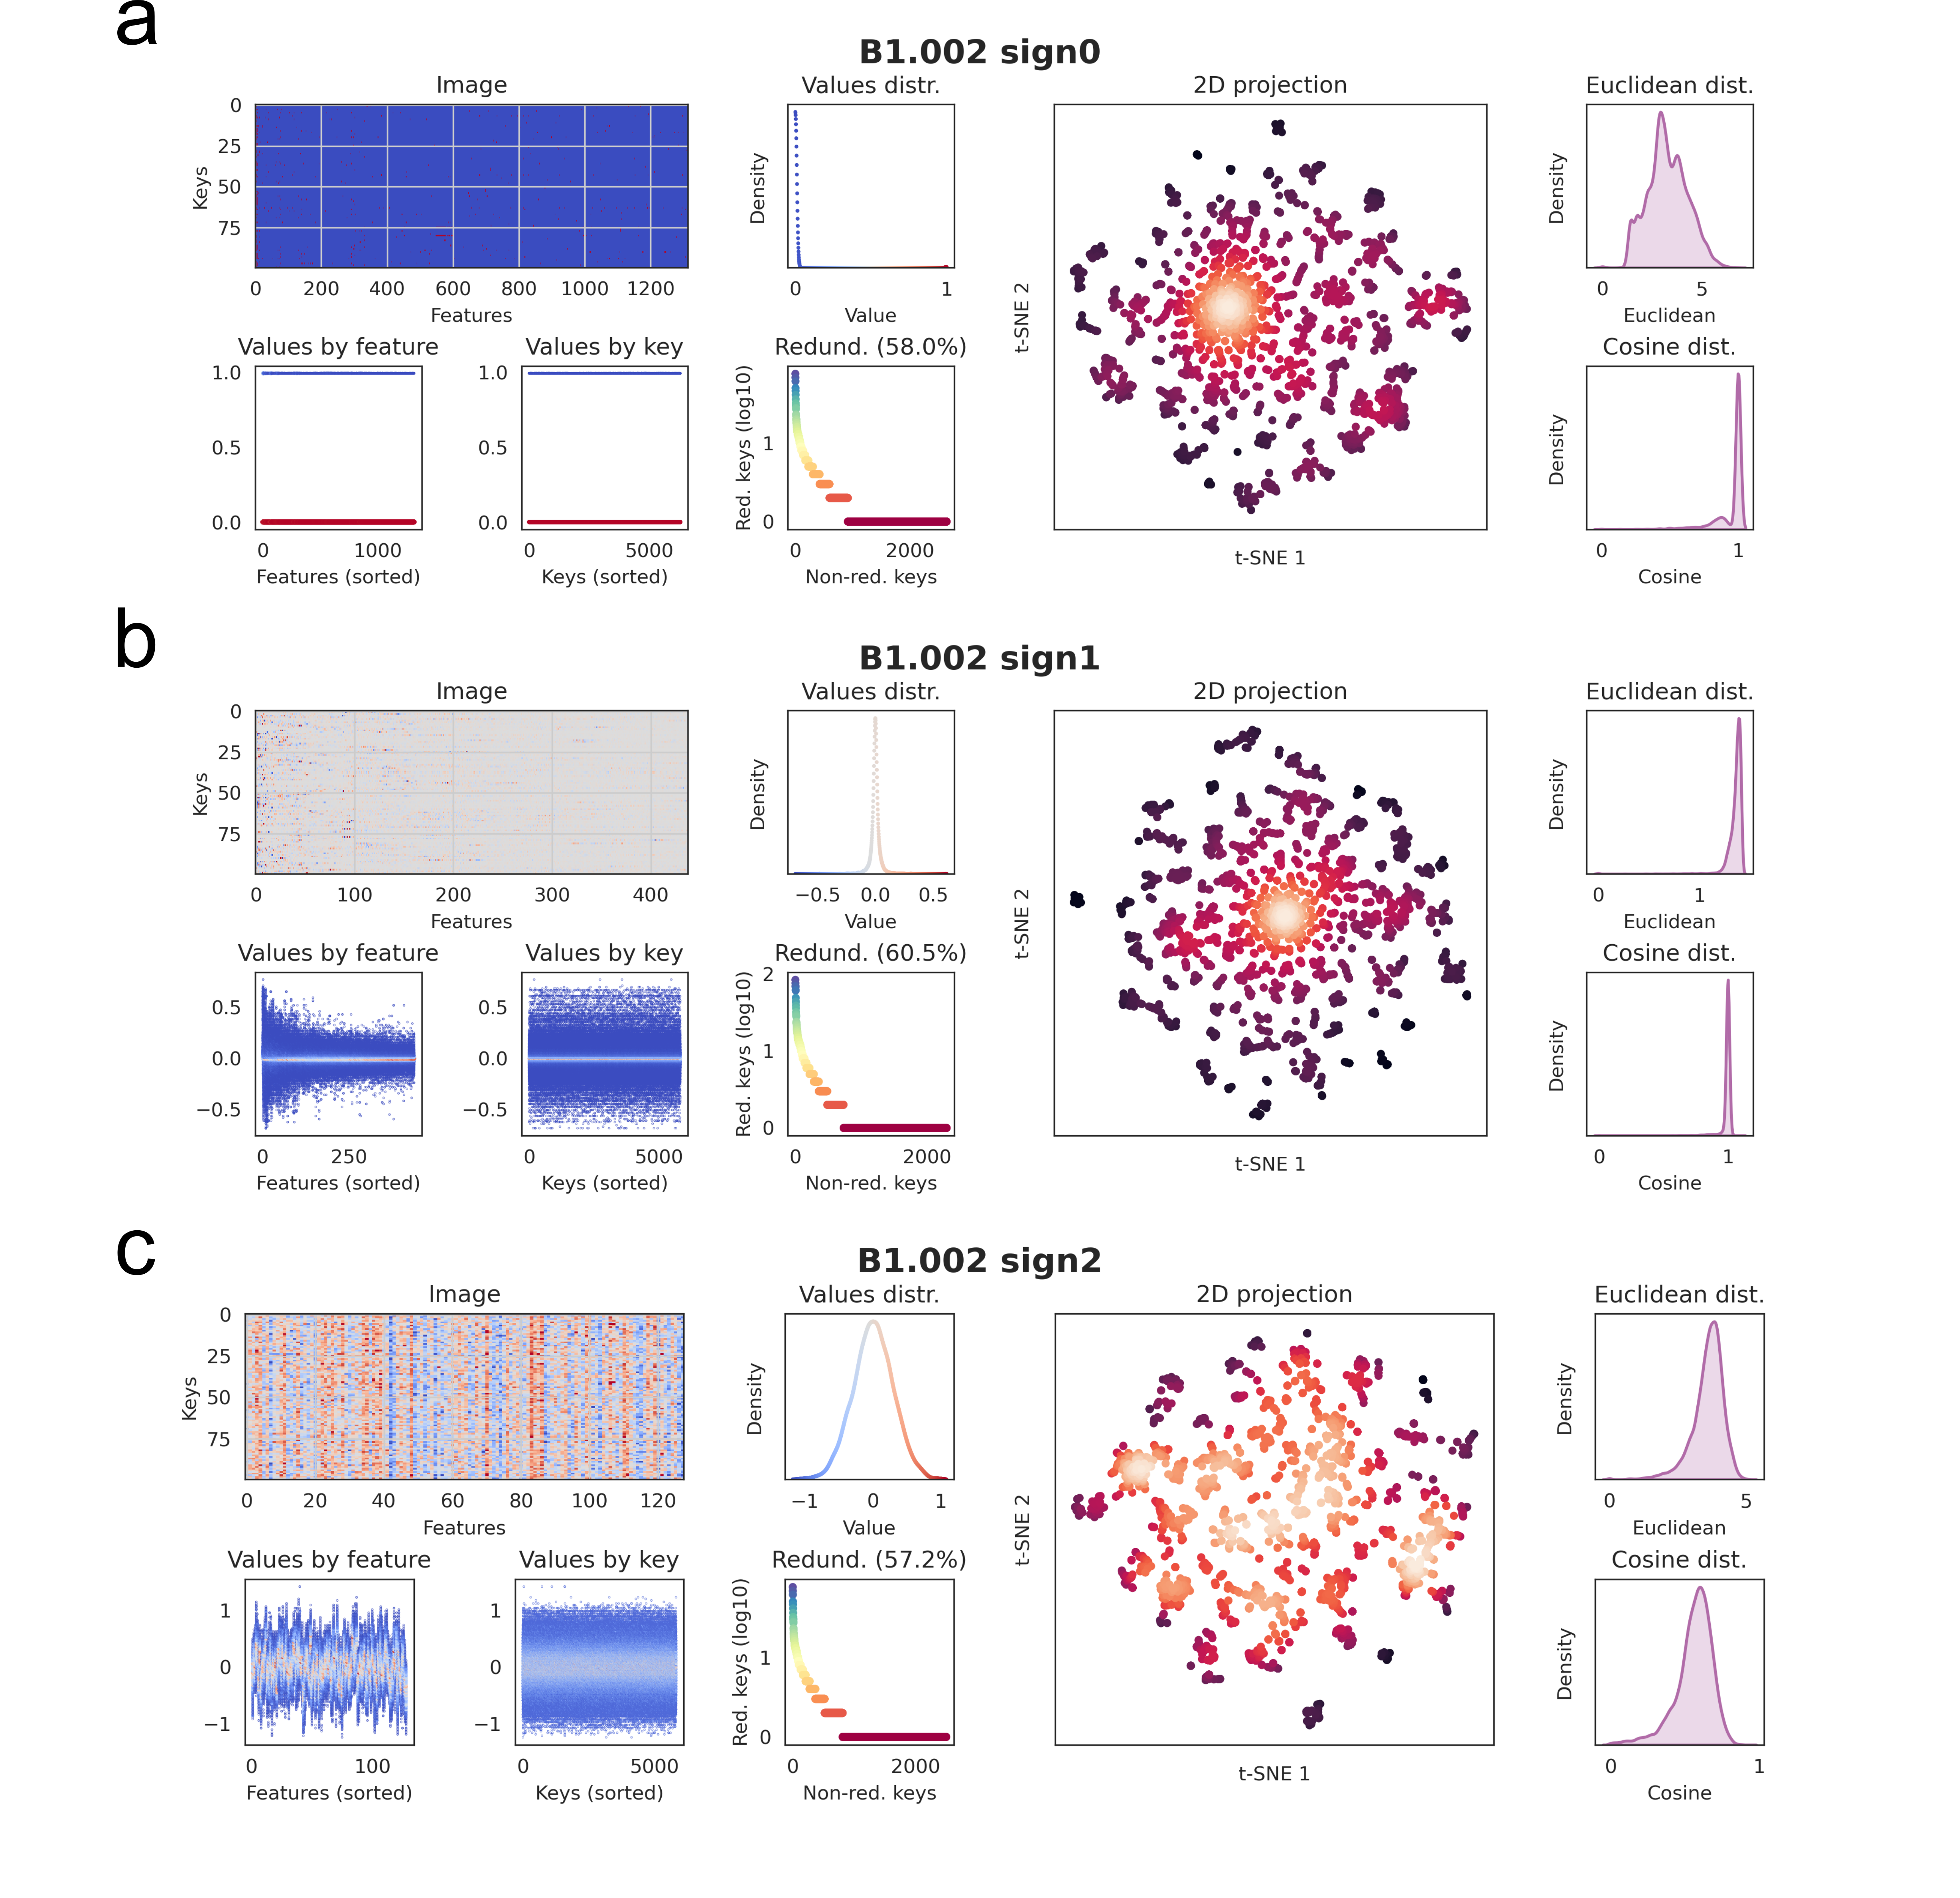
\includegraphics[width=0.8\linewidth]{figures/Protocols/Supplementary/B1.002_v2.png}
  \caption{
    Diagnosis plots for the B1.002 space.
    \textbf{a)} type 0 signatures,
    \textbf{b)} type I signatures,
    \textbf{c)} type II signatures. For further information about diagnosis plots, please see the \hyperref[Supplementary_Protocols_Diagnosis]{Supplementary Information}.
  }
  \label{Protocols_FigS1}
\end{figure}


\begin{figure}[htbp]
  \centering
  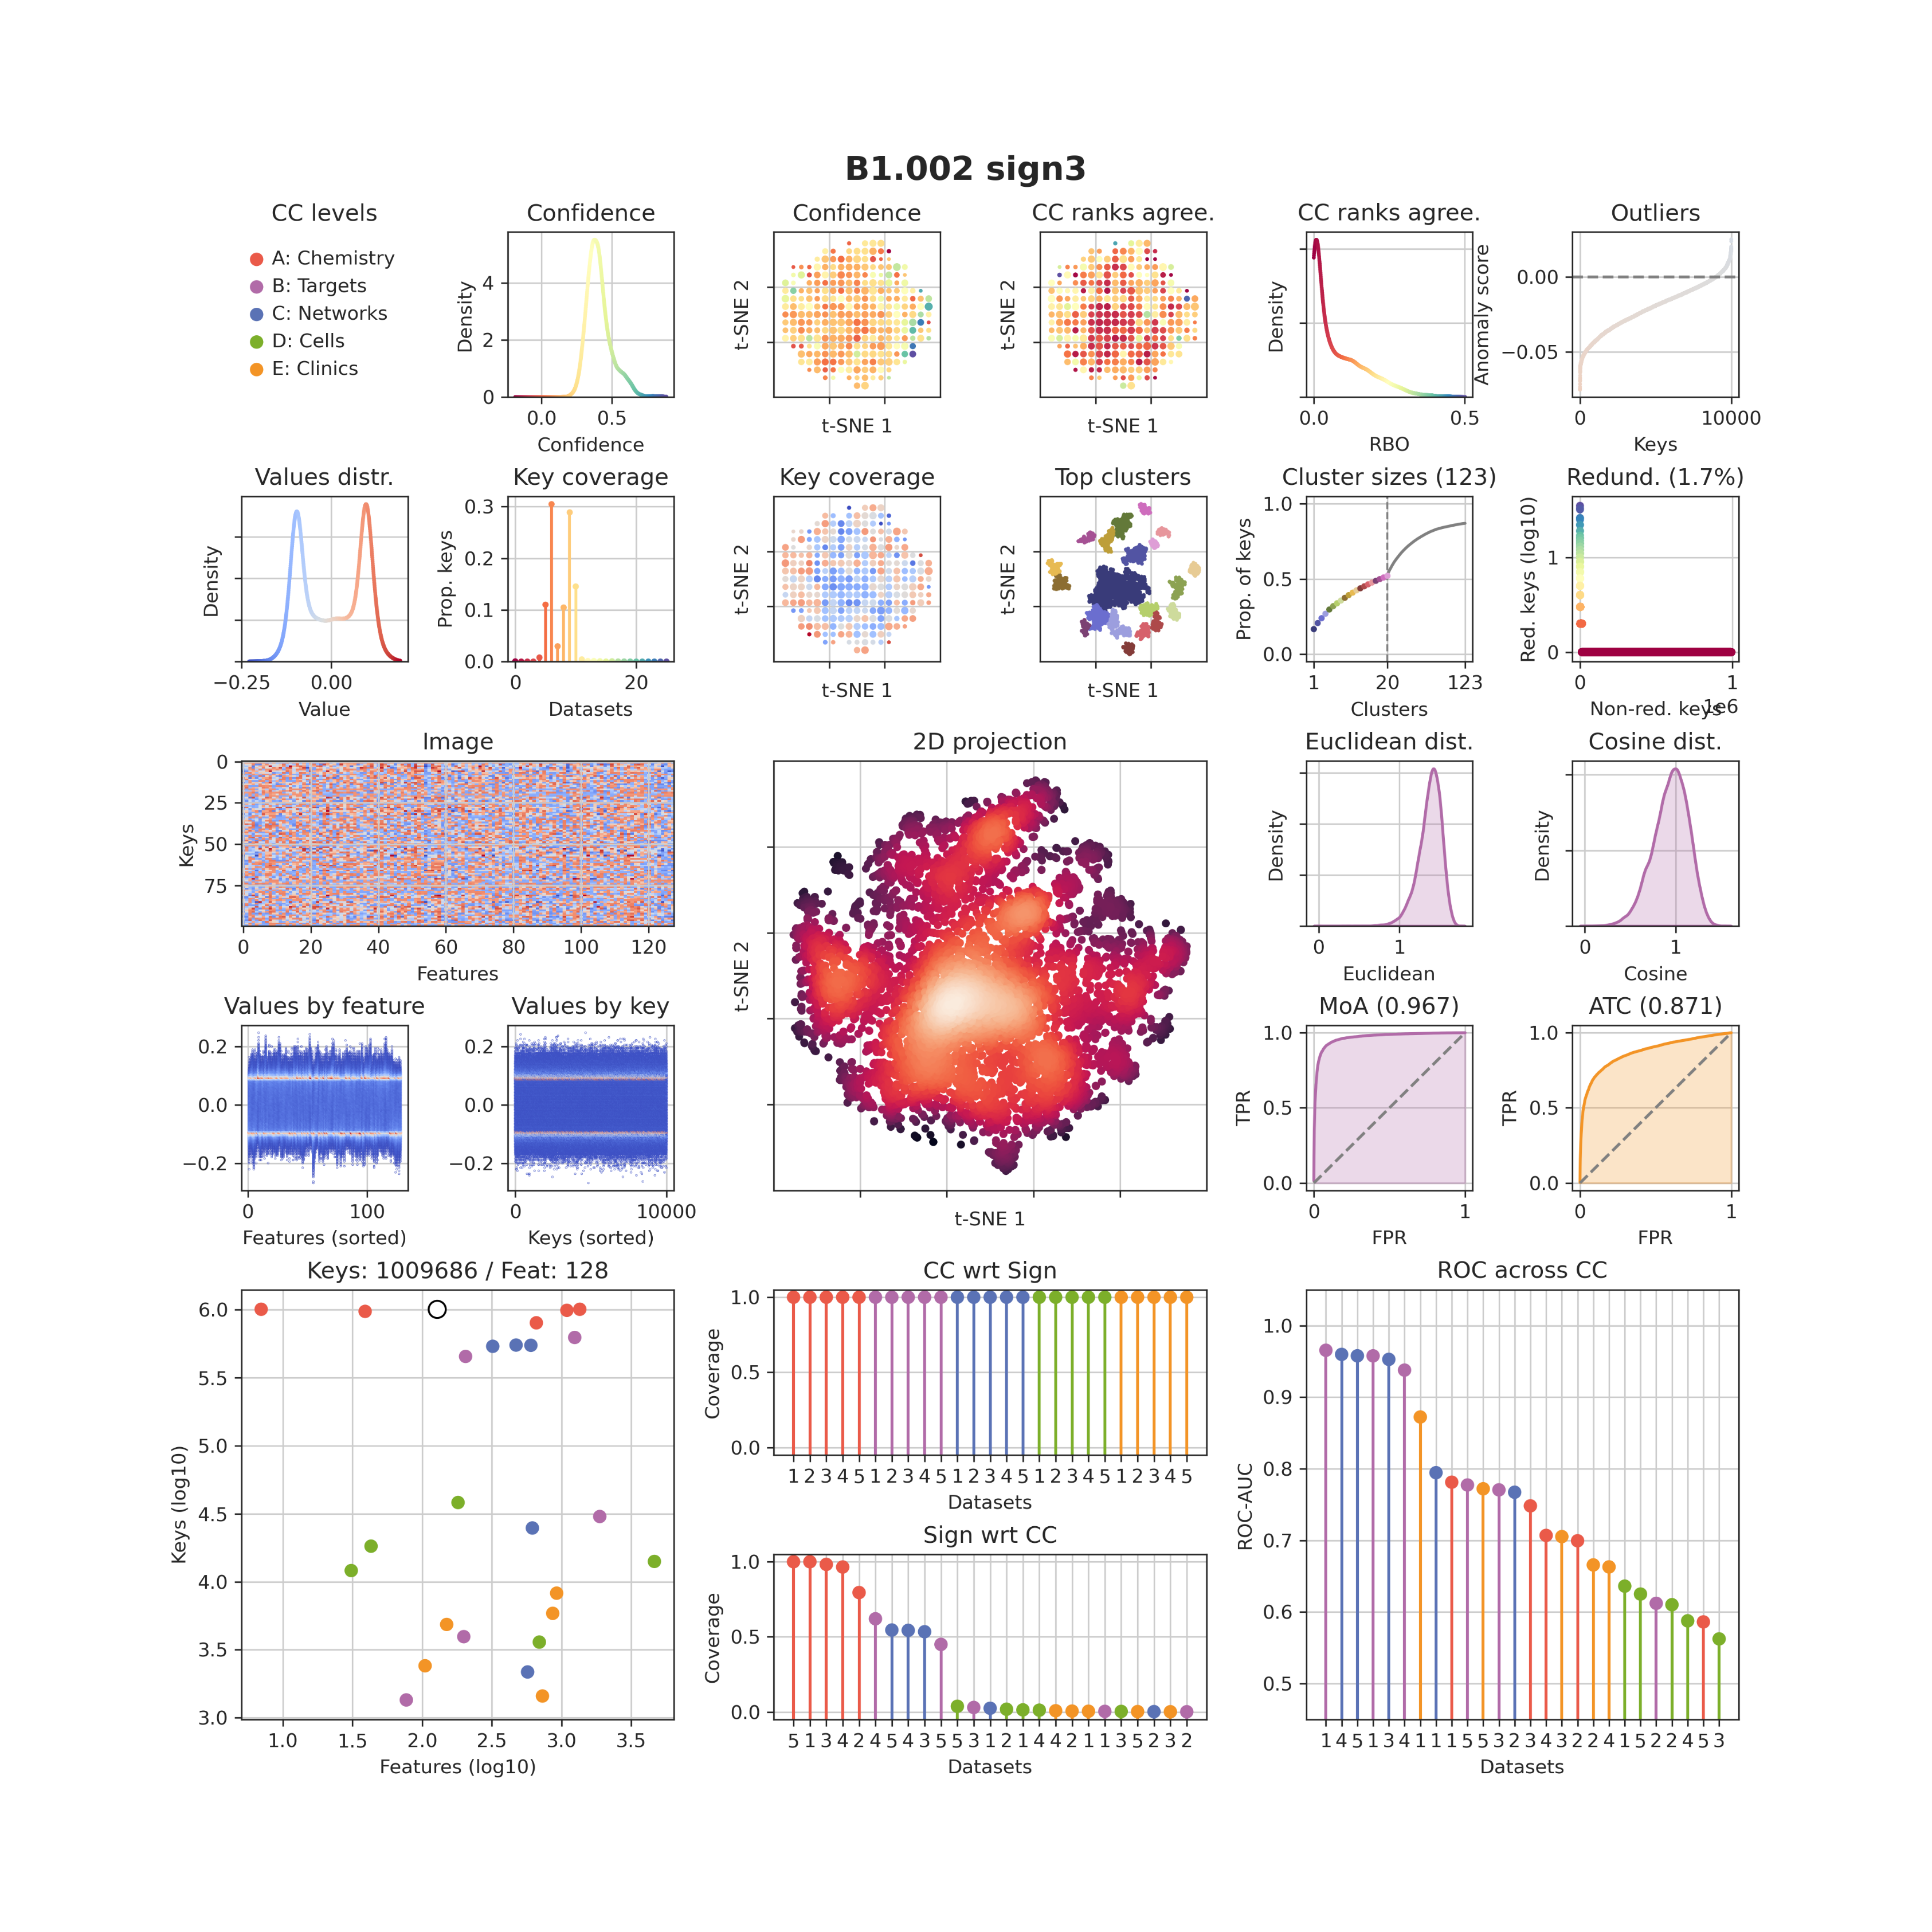
\includegraphics[width=1\linewidth]{figures/Protocols/Supplementary/B1_medium.sign3_v2.png}
  \caption{
    Extended diagnosis plots for B1.002 type III signatures. For further information about diagnosis plots, please see the \hyperref[Supplementary_Protocols_Diagnosis]{Supplementary Information} and check our \href{https://gitlabsbnb.irbbarcelona.org/packages/protocols}{Gitlab repository}.
  }
  \label{Protocols_FigS2}
\end{figure}


\begin{figure}[htbp]
  \centering
  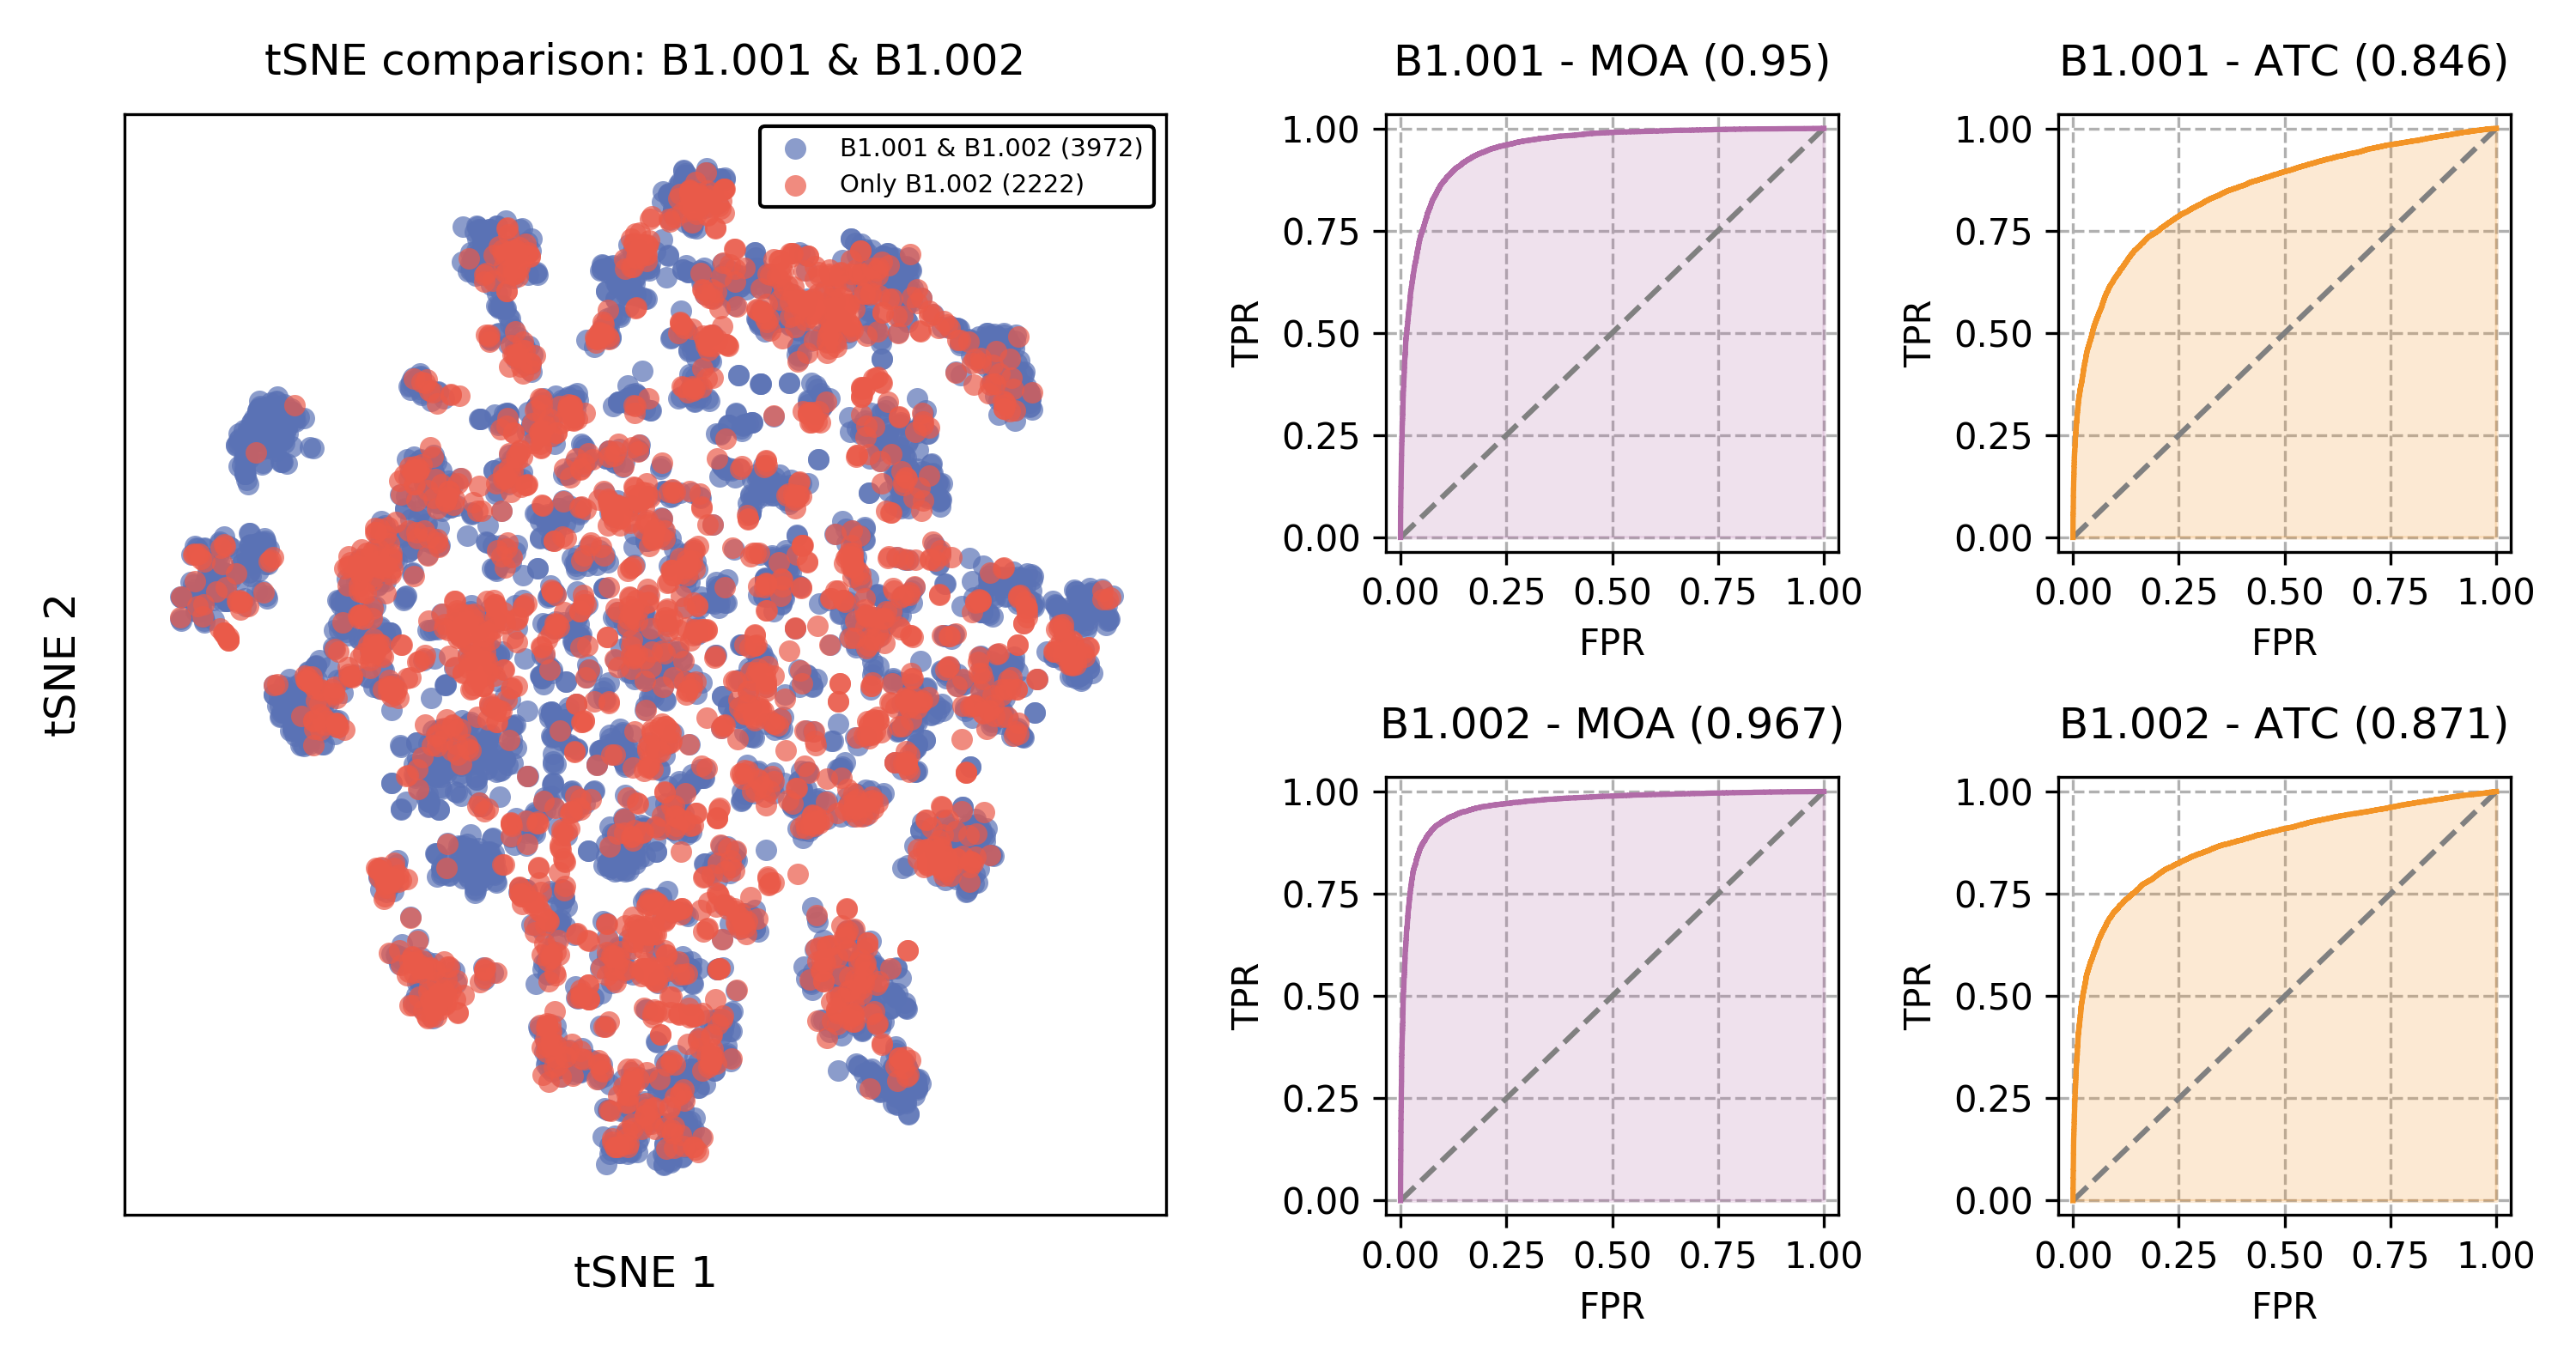
\includegraphics[width=1\linewidth]{figures/Protocols/Supplementary/FigS3.png}
  \caption{
    Comparison between B1.001 and B1.002. Left: 2D tSNE representation of B1.001 and B1.002 type III signatures having a corresponding type 0 signature in B1.001 and B1.002, respectively. Right: recapitulation of MOA (B1.001 type 0 signatures, purple) and ATC (E1.001 type 0 signatures, orange) using B1.001 (top) and B1.002 (bottom) type III signatures. 
  }
  \label{Protocols_FigS3}
\end{figure}


\begin{figure}[htbp]
  \centering
  \includegraphics[width=1\linewidth]{figures/Protocols/Supplementary/D1.002_v2.png}
  \caption{
    Diagnosis plots for the D1.002 space
    \textbf{a)} type 0 signatures,
    \textbf{b)} type I signatures,
    \textbf{c)} type II signatures. For further information about diagnosis plots, please see the \hyperref[Supplementary_Protocols_Diagnosis]{Supplementary Information}.
  }
  \label{Protocols_FigS4}
\end{figure}

\begin{figure}[htbp]
  \centering
  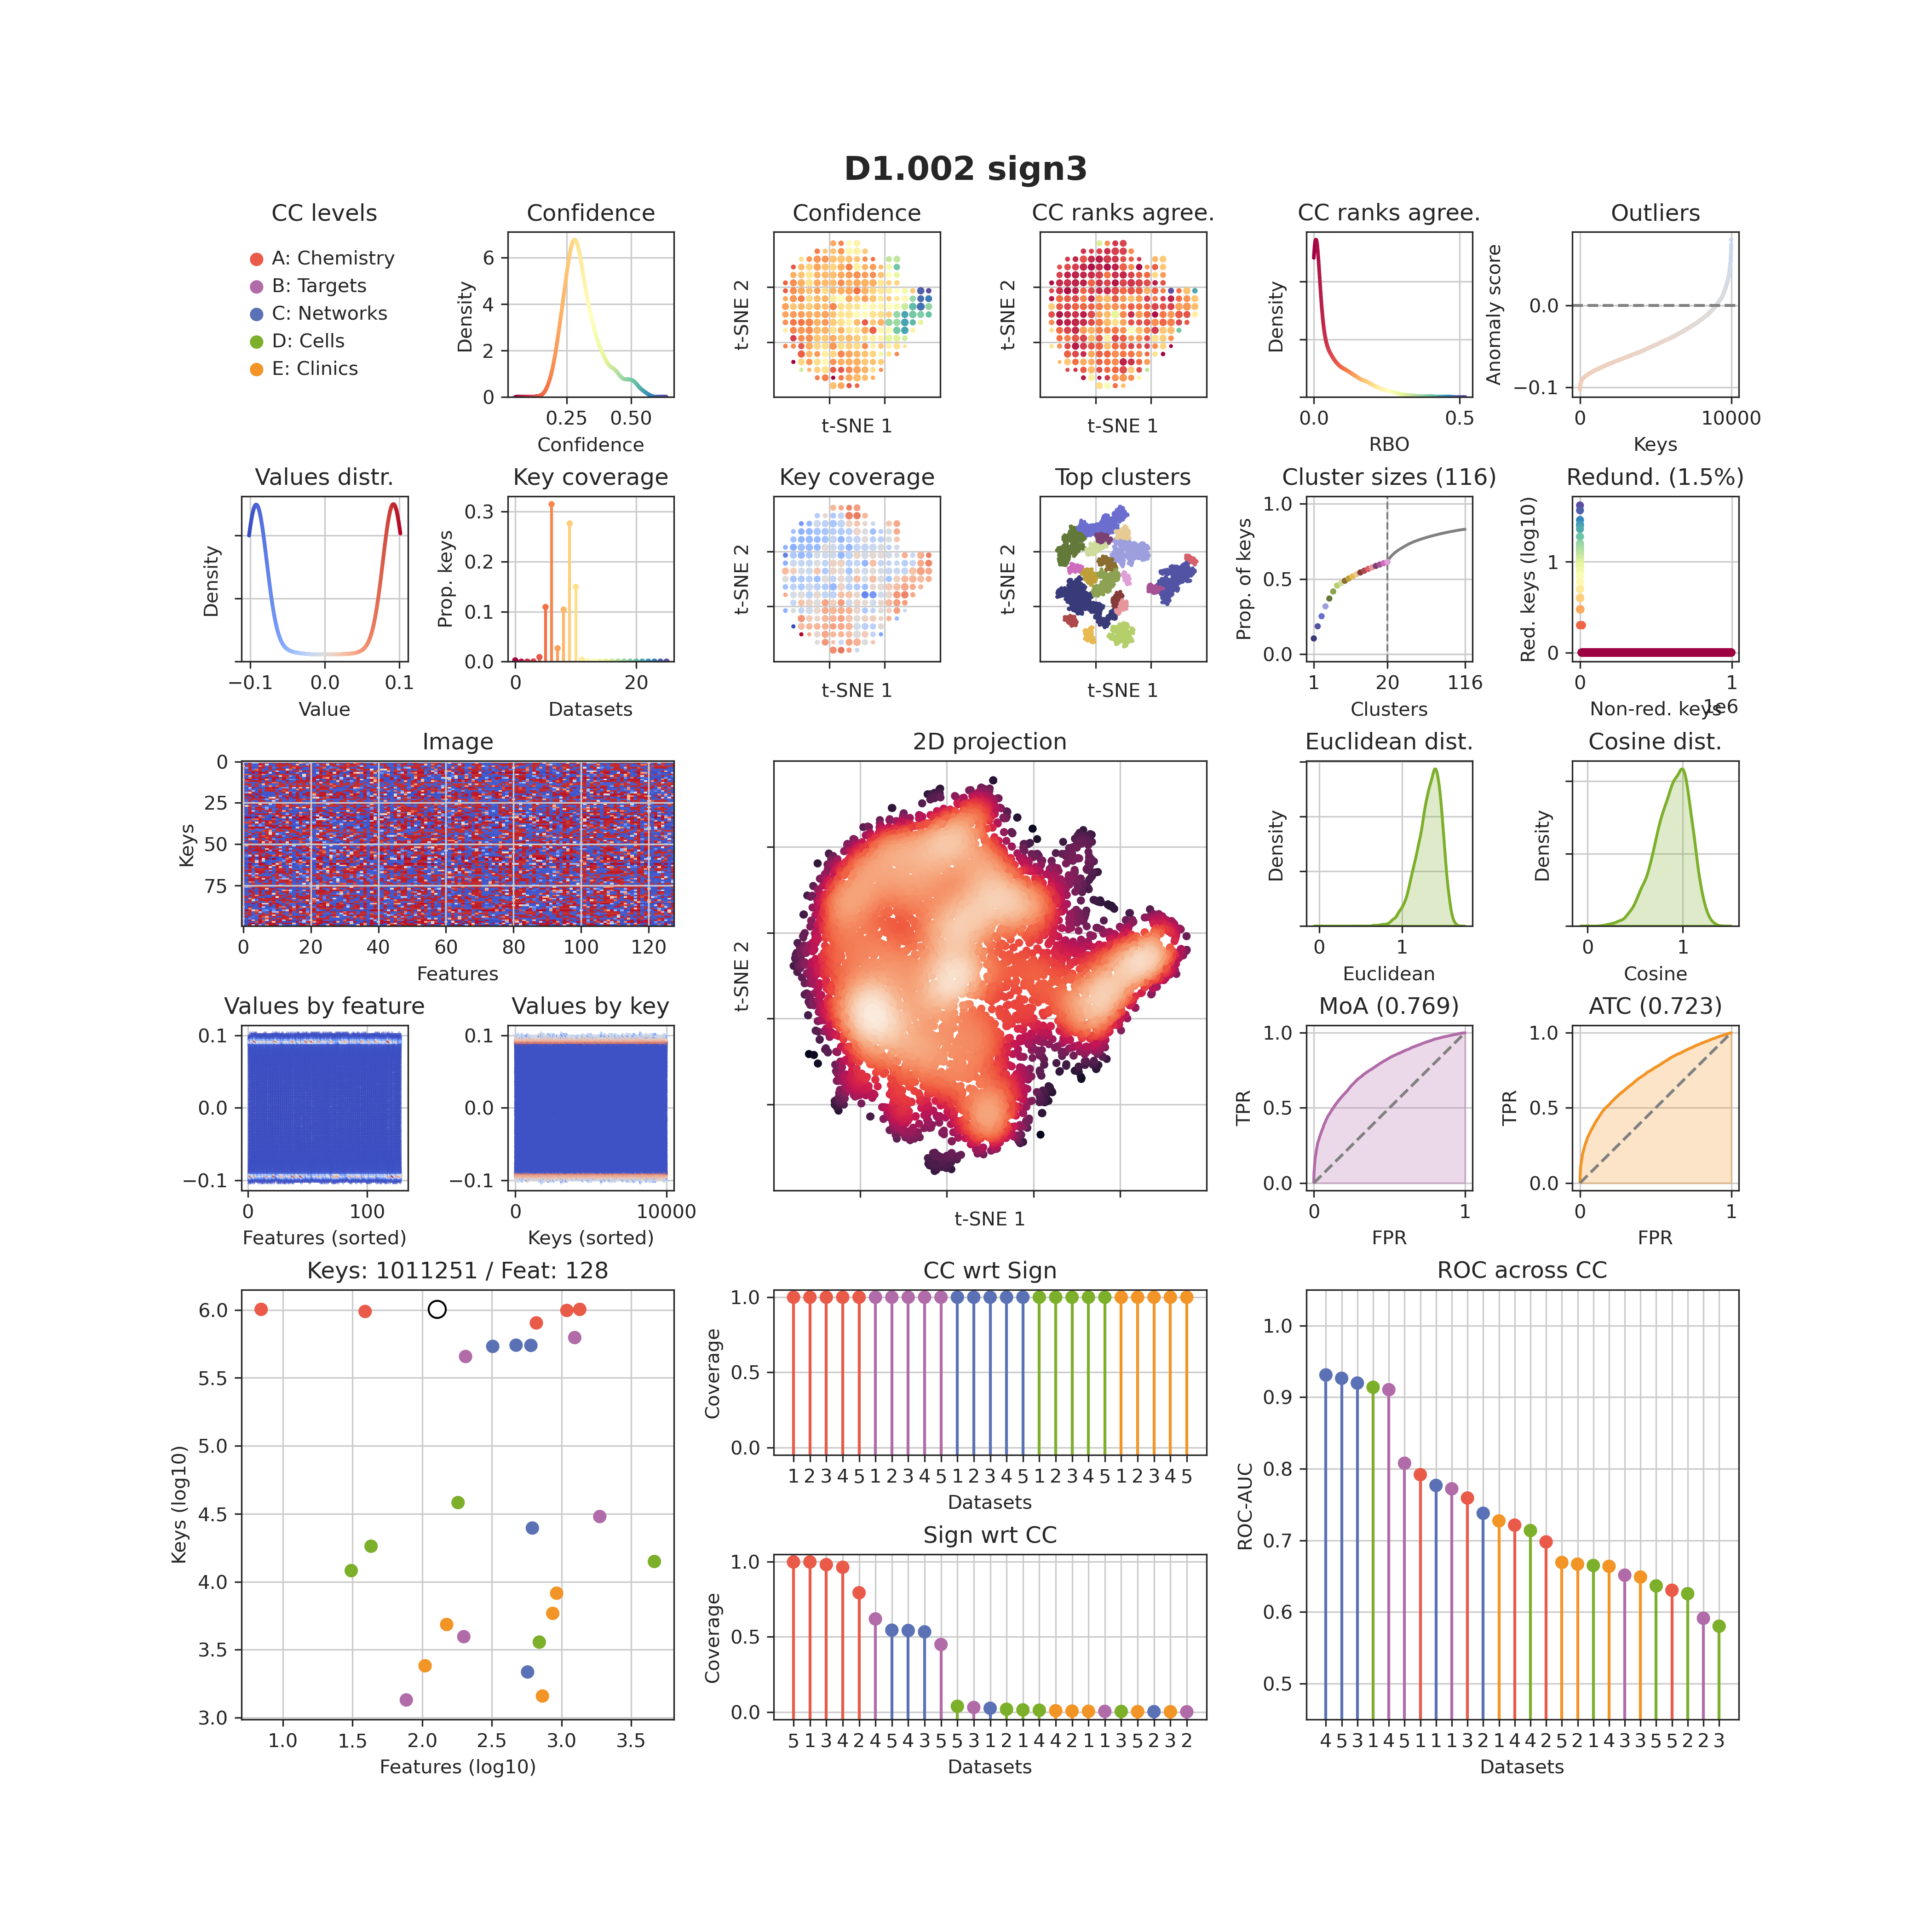
\includegraphics[width=1\linewidth]{figures/Protocols/Supplementary/D1.002_sign3_local_CC_D1_sign0_medium.png}
  \caption{
    Extended diagnosis plots for D1.002 type III signatures. For further information about diagnosis plots, please see the \hyperref[Supplementary_Protocols_Diagnosis]{Supplementary Information} and check our \href{https://gitlabsbnb.irbbarcelona.org/packages/protocols}{Gitlab repository}.
  }
  \label{Protocols_FigS5}
\end{figure}

\begin{figure}[htbp]
  \centering
  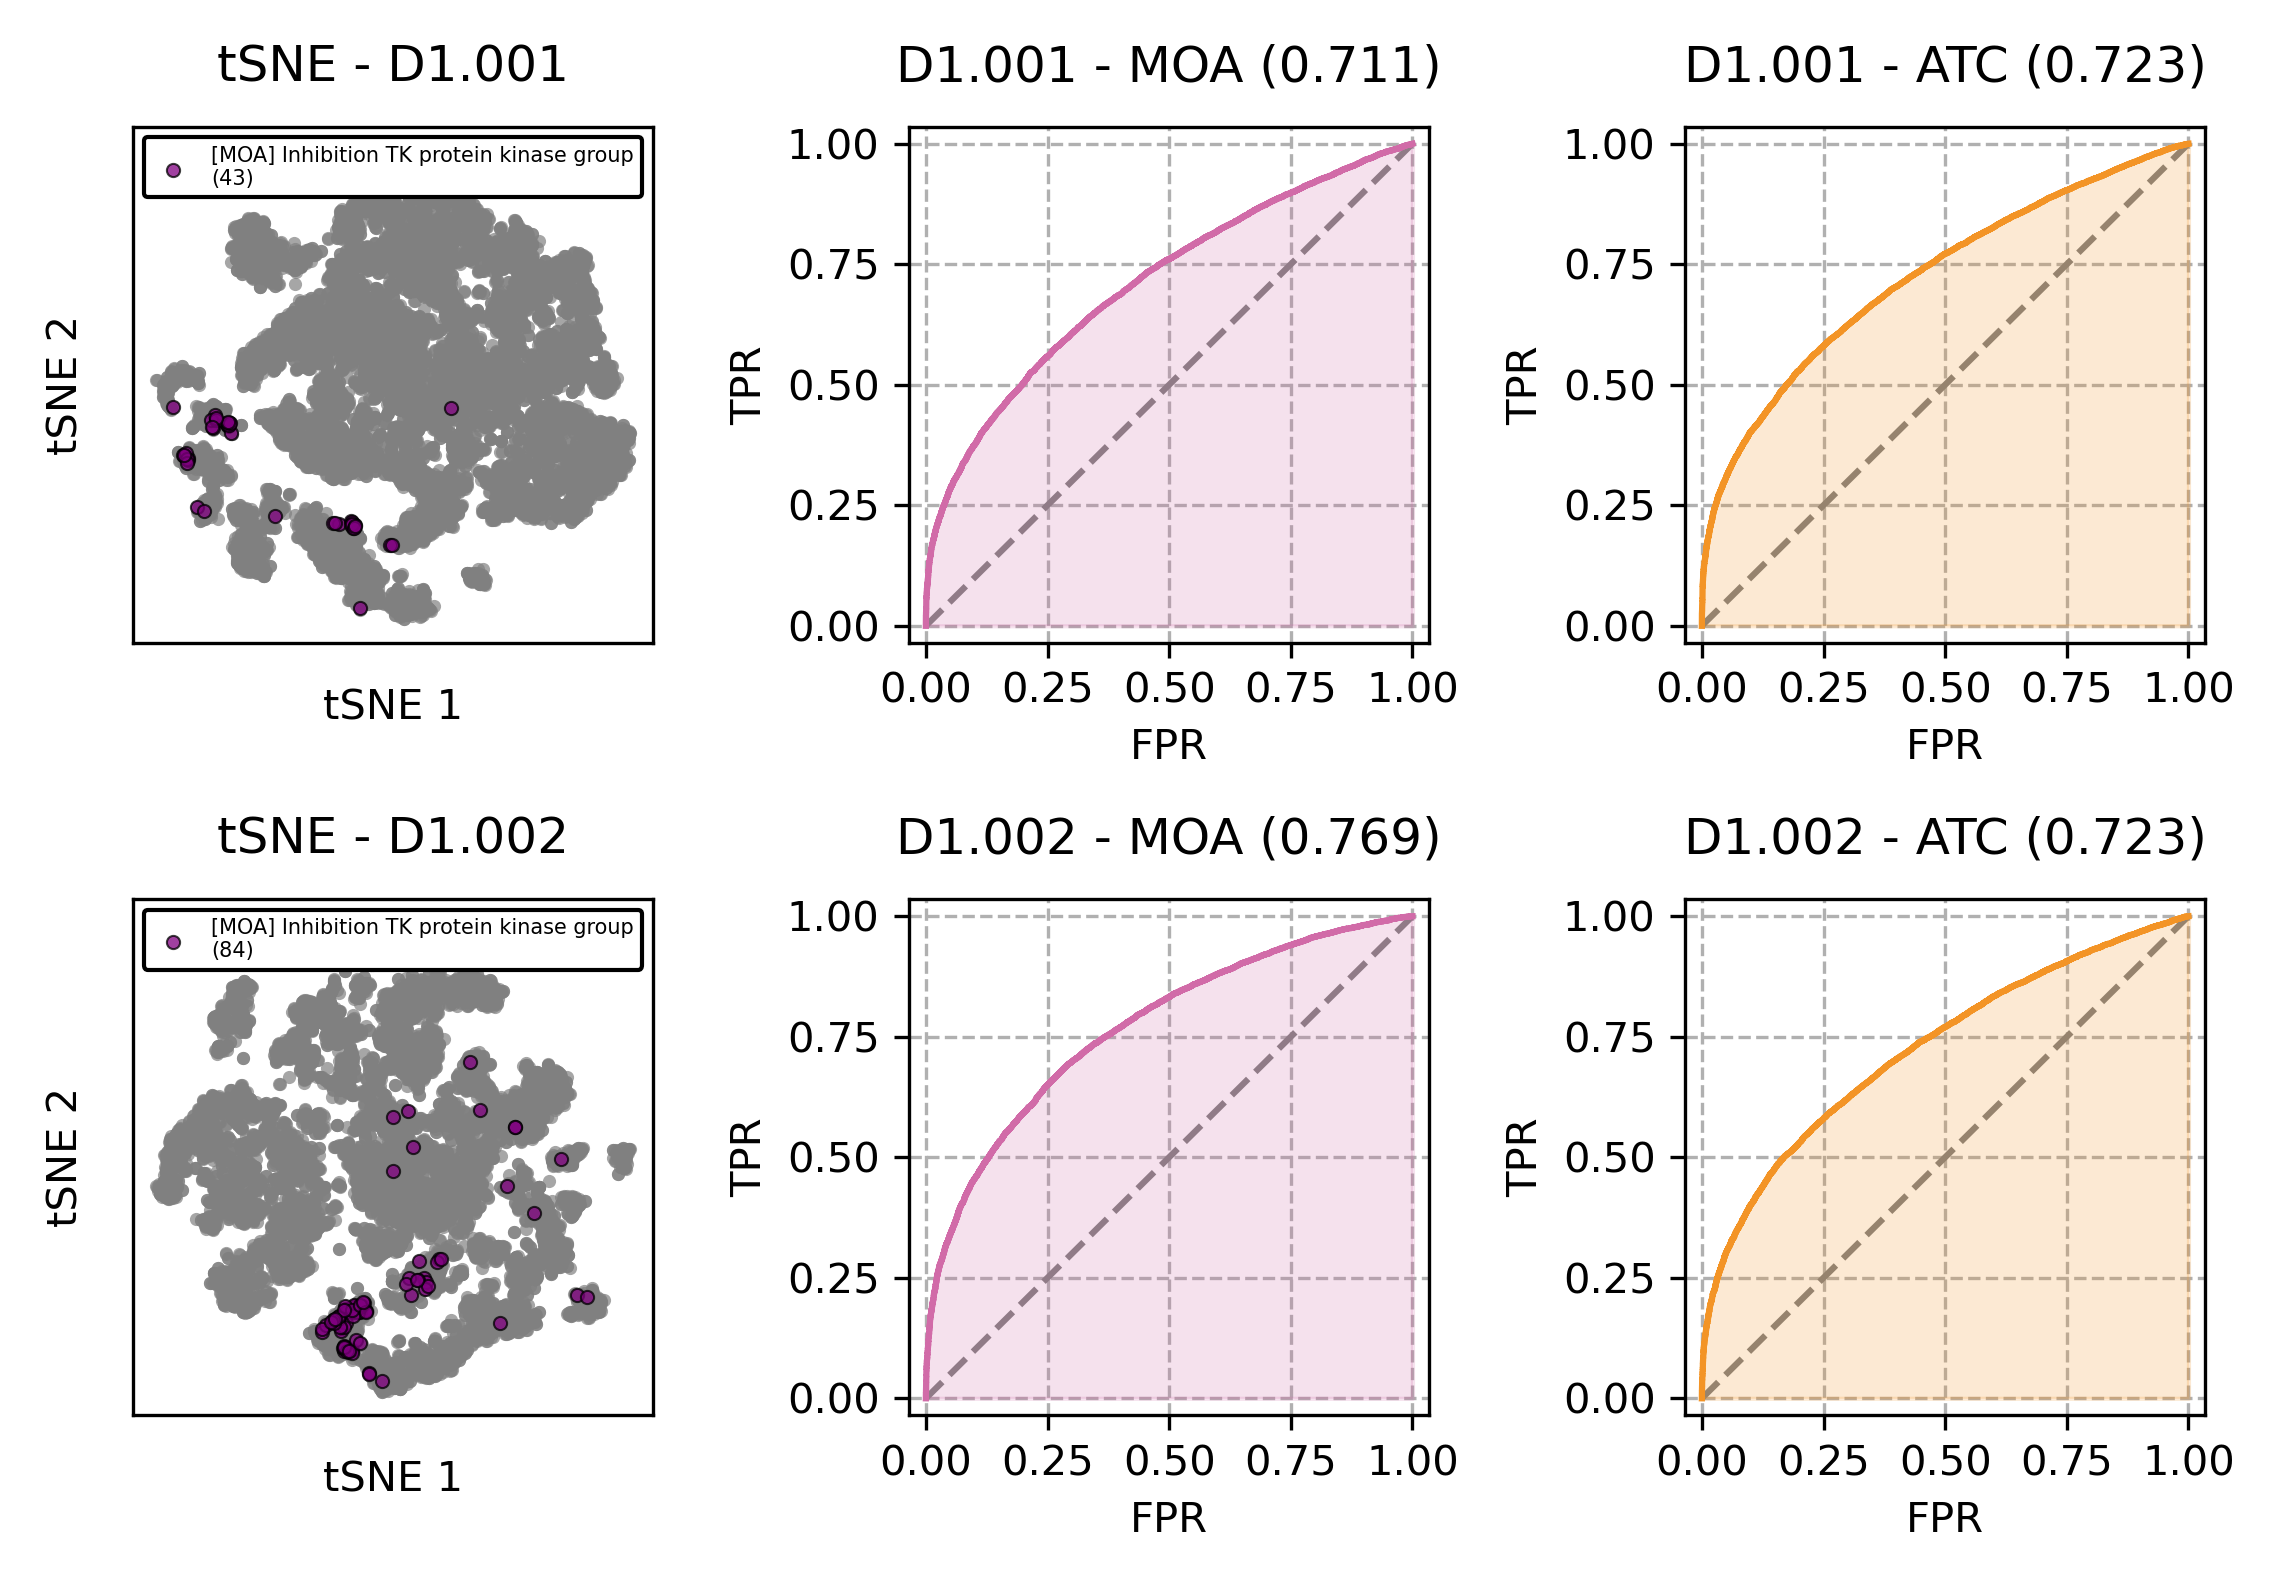
\includegraphics[width=1\linewidth]{figures/Protocols/Supplementary/FigS6.png}
  \caption{
    Comparison between D1.001 and D1.002. Left: 2D tSNE representation of D1.001 (top) and D1.002 (bottom) type III signatures having a corresponding type 0 signature in D1.001 and D1.002, respectively. Points highlighted in purple correspond to compounds related to the inhibition of the TK protein group.  Center and right: recapitulation of MOA (B1.001 type 0 signatures, purple) and ATC (E1.001 type 0 signatures, orange) using D1.001 (top) and D1.002 (bottom) type III signatures.  
  }
  \label{Protocols_FigS6}
\end{figure}


\begin{figure}[htbp]
  \centering
  \includegraphics[width=1\linewidth]{figures/Protocols/Supplementary/D6.001_v2.png}
  \caption{
    Diagnosis plots for the D6.001 space
    \textbf{a)} type 0 signatures,
    \textbf{b)} type I signatures,
    \textbf{c)} type II signatures. For further information about diagnosis plots, please see the \hyperref[Supplementary_Protocols_Diagnosis]{Supplementary Information}.
  }
  \label{Protocols_FigS7}
\end{figure}


\begin{figure}[htbp]
  \centering
  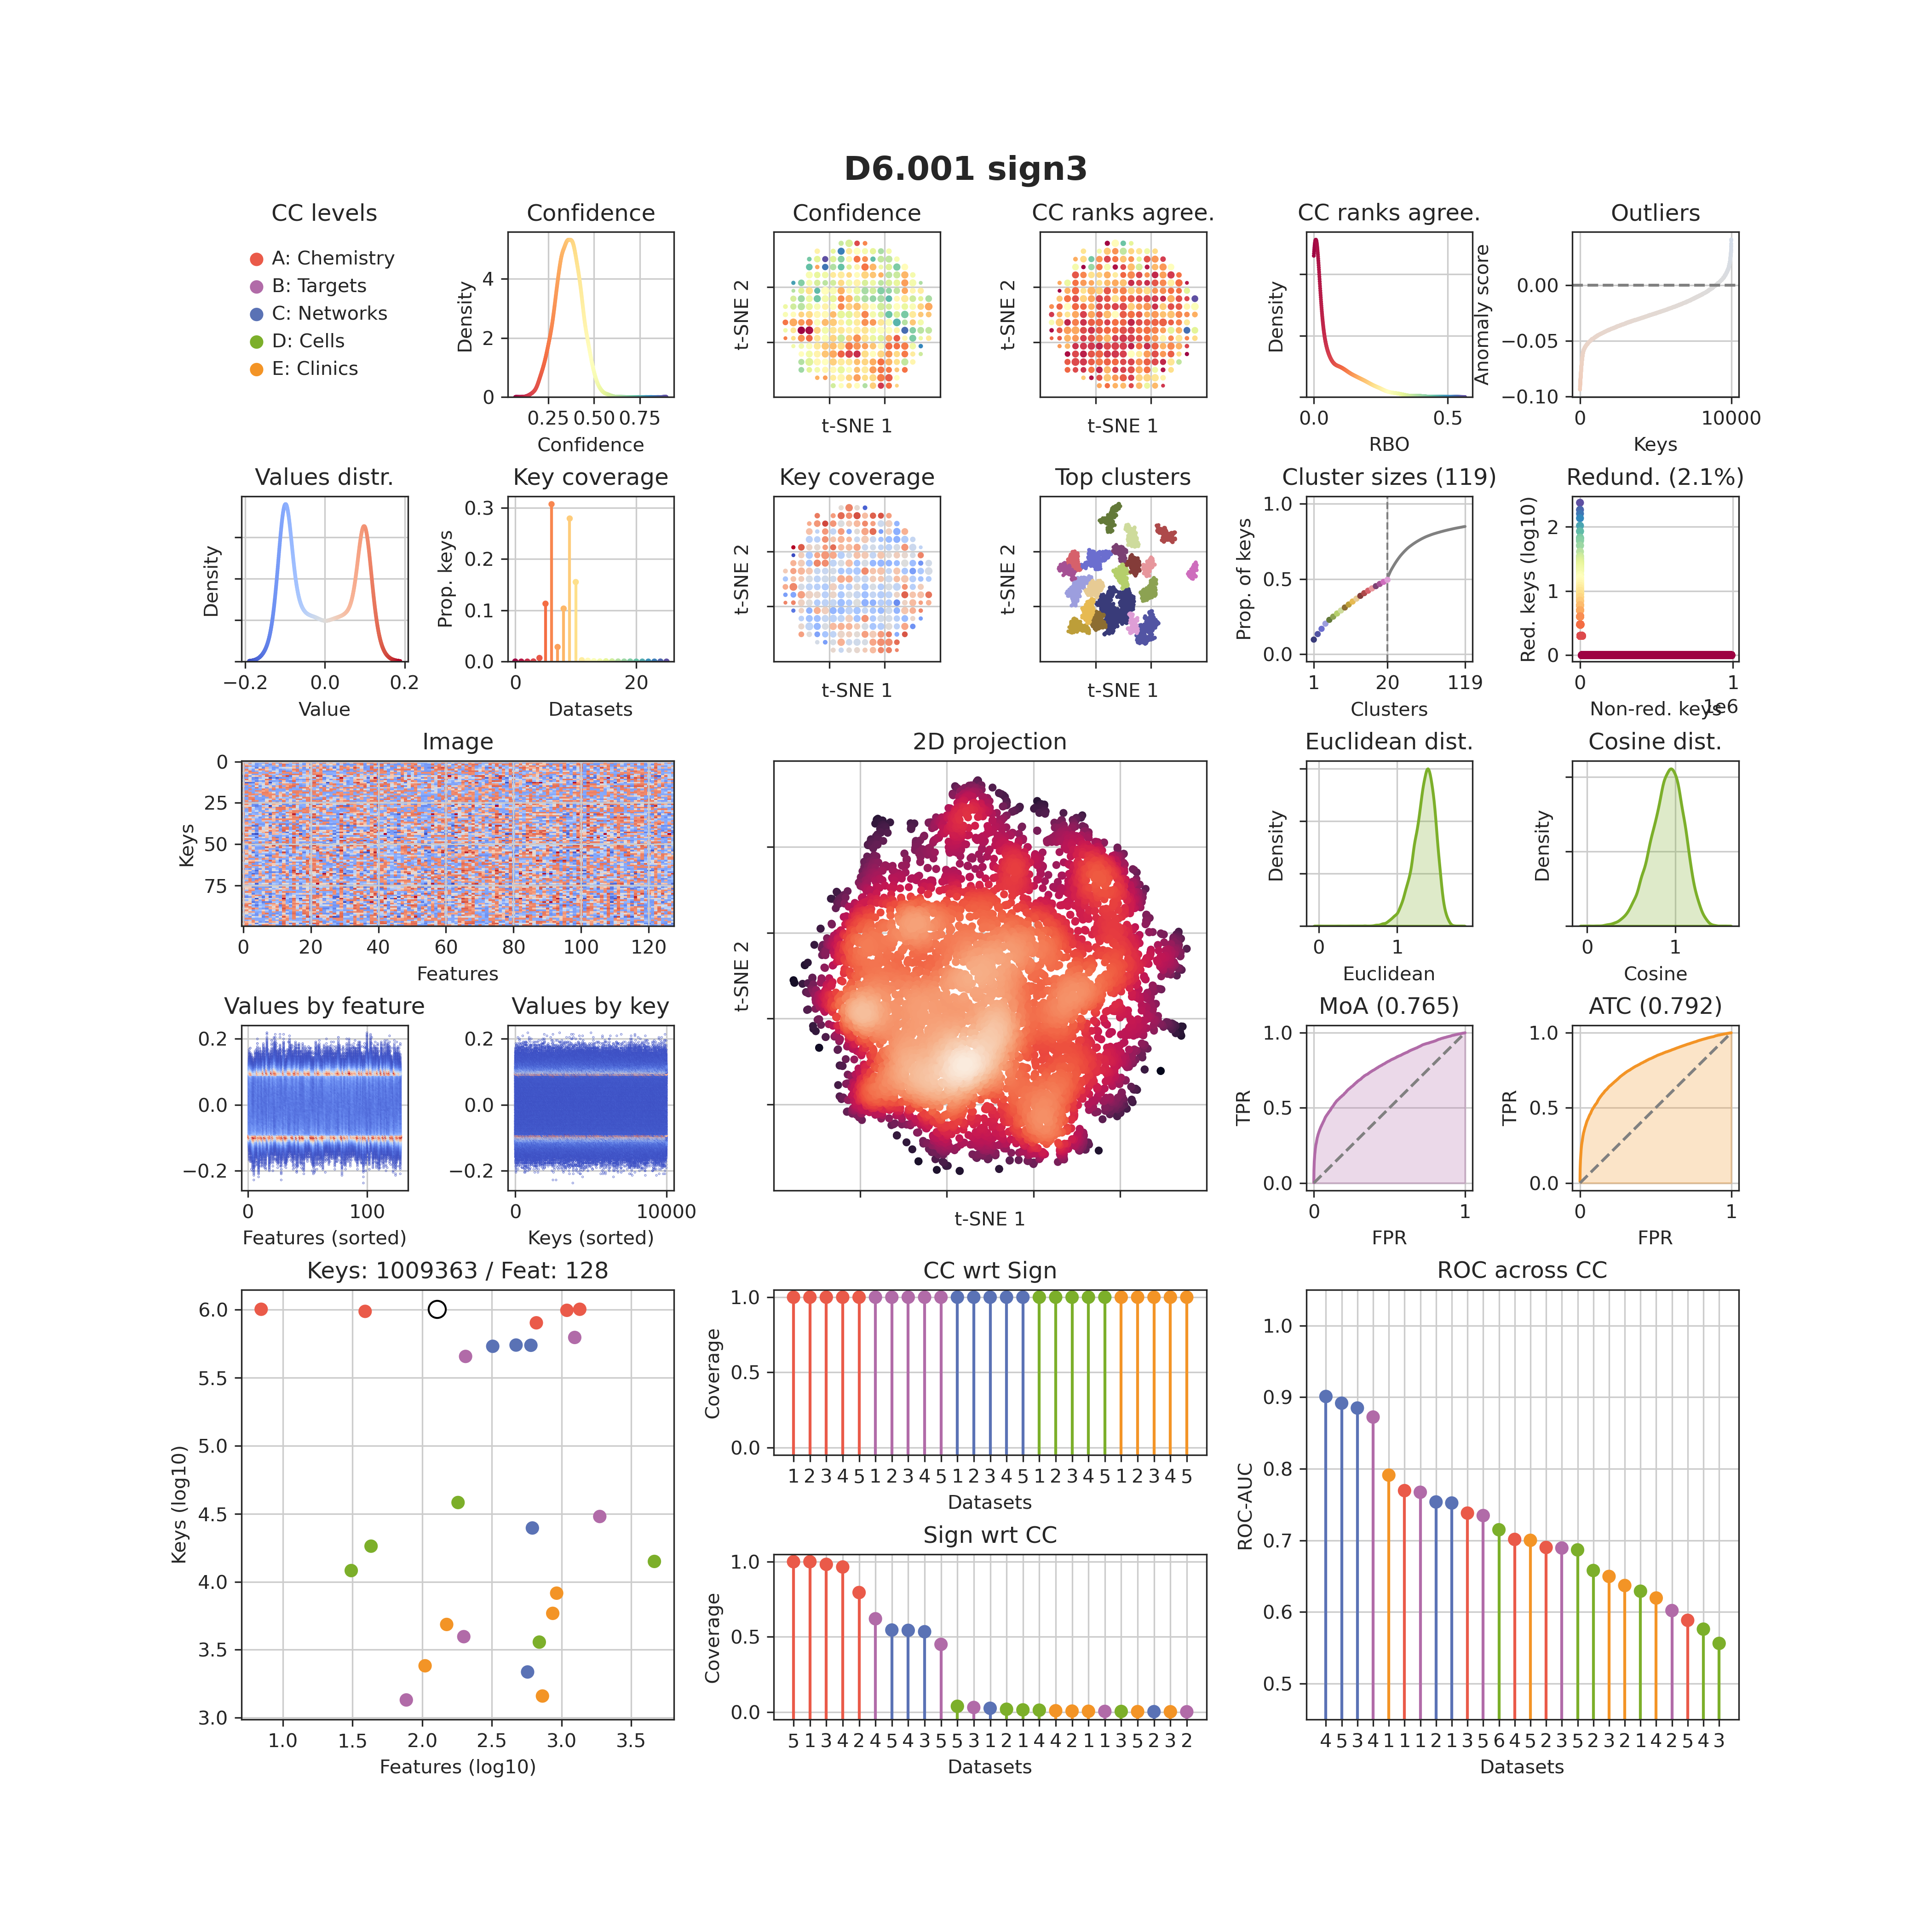
\includegraphics[width=1\linewidth]{figures/Protocols/Supplementary/D6.001_sign3_local_CC_D6_sign0_medium.png}
  \caption{
    Extended diagnosis plots for D6.001 type III signatures. For further information about diagnosis plots, please see the \hyperref[Supplementary_Protocols_Diagnosis]{Supplementary Information} and check our \href{https://gitlabsbnb.irbbarcelona.org/packages/protocols}{Gitlab repository}.
  }
  \label{Protocols_FigS8}
\end{figure}


\begin{figure}[htbp]
  \centering
  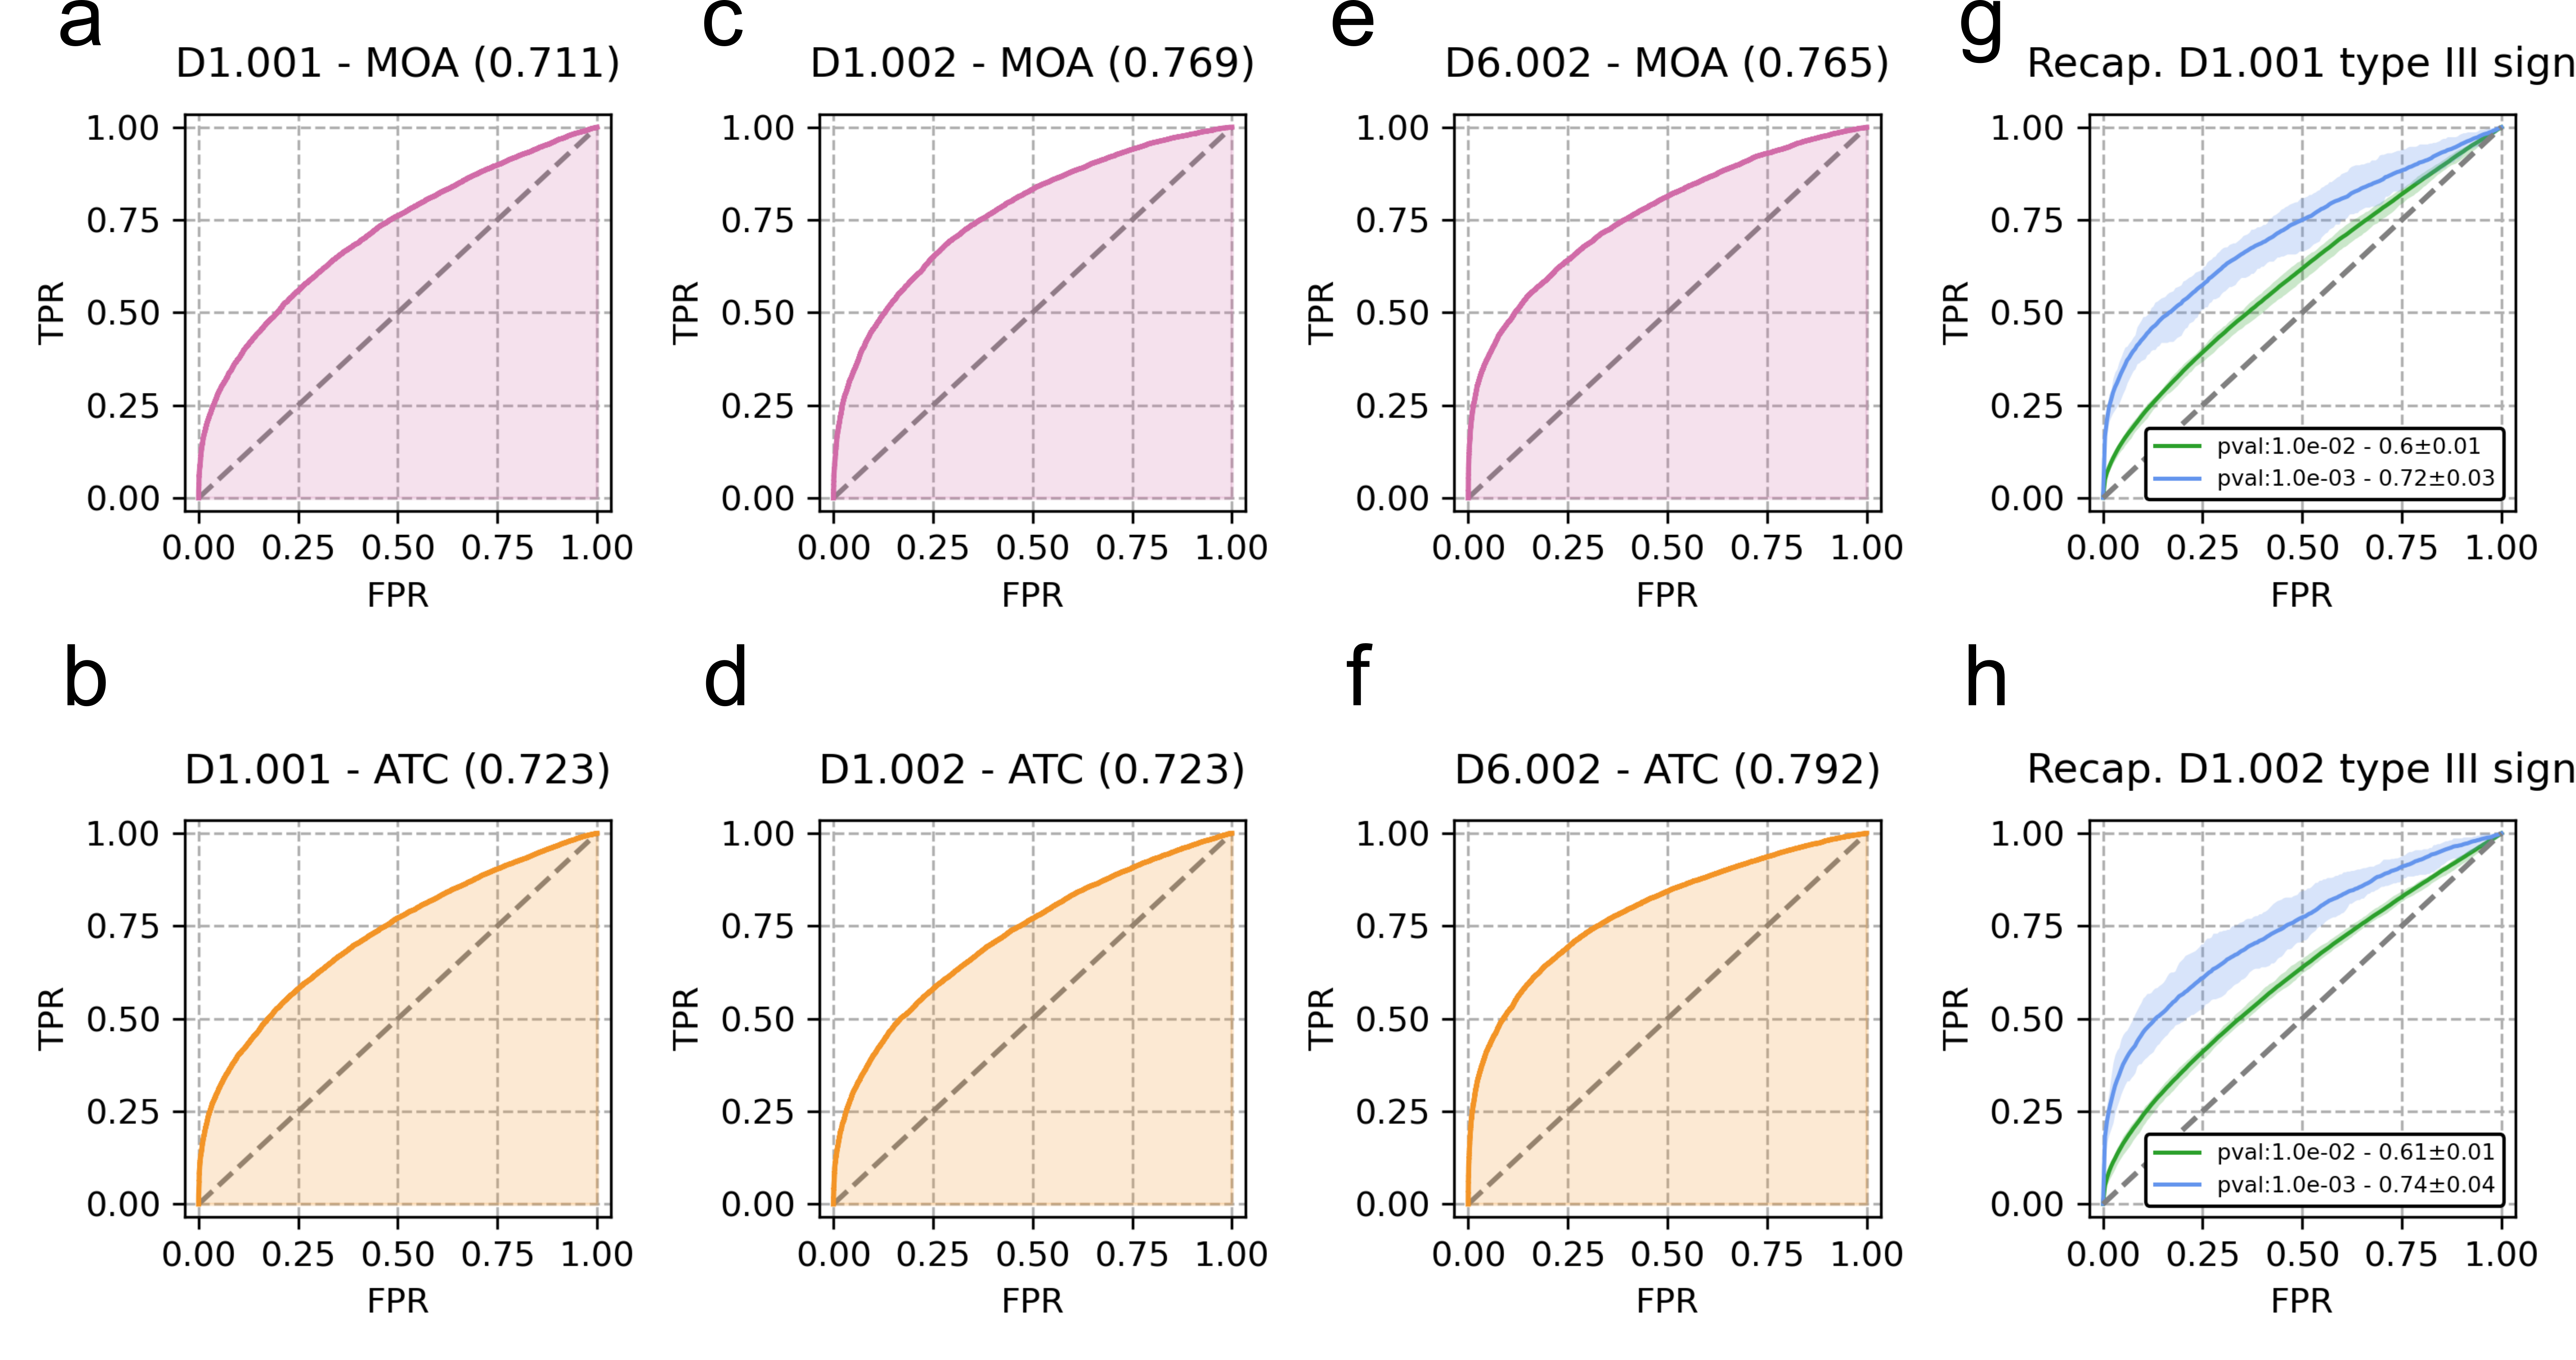
\includegraphics[width=1\linewidth]{figures/Protocols/Supplementary/FigS9_v2.png}
  \caption{
    Comparison between D1.001, D1.002 and D6.001.
    \textbf{a)} Recapitulation of MoA (B1.001 type 0 signatures, purple) using D1.001 type III signatures.
    \textbf{b)} Recapitulation of ATC (E1.001 type 0 signatures, orange) using D1.001 type III signatures.
    \textbf{c)} Recapitulation of MoA (B1.001 type 0 signatures, purple) using D1.002 type III signatures.
    \textbf{d)} Recapitulation of ATC (E1.001 type 0 signatures, orange) using D1.002 type III signatures. 
    \textbf{e)} Recapitulation of MoA (B1.001 type 0 signatures, purple) using D6.001 type III signatures.
    \textbf{f)} Recapitulation of ATC (E1.001 type 0 signatures, orange) using D6.001 type III signatures.
    \textbf{g)} Recapitulation of kNN at D1.001 type III signature level using D6.001 type III signatures at p-values 0.01 and 0.001.
    \textbf{h)} Recapitulation of NN at D1.002 type III signature level using D6.001 type III signatures at p-values 0.01 and 0.001.
  }
  \label{Protocols_FigS9}
\end{figure}


\begin{figure}[htbp]
  \centering
  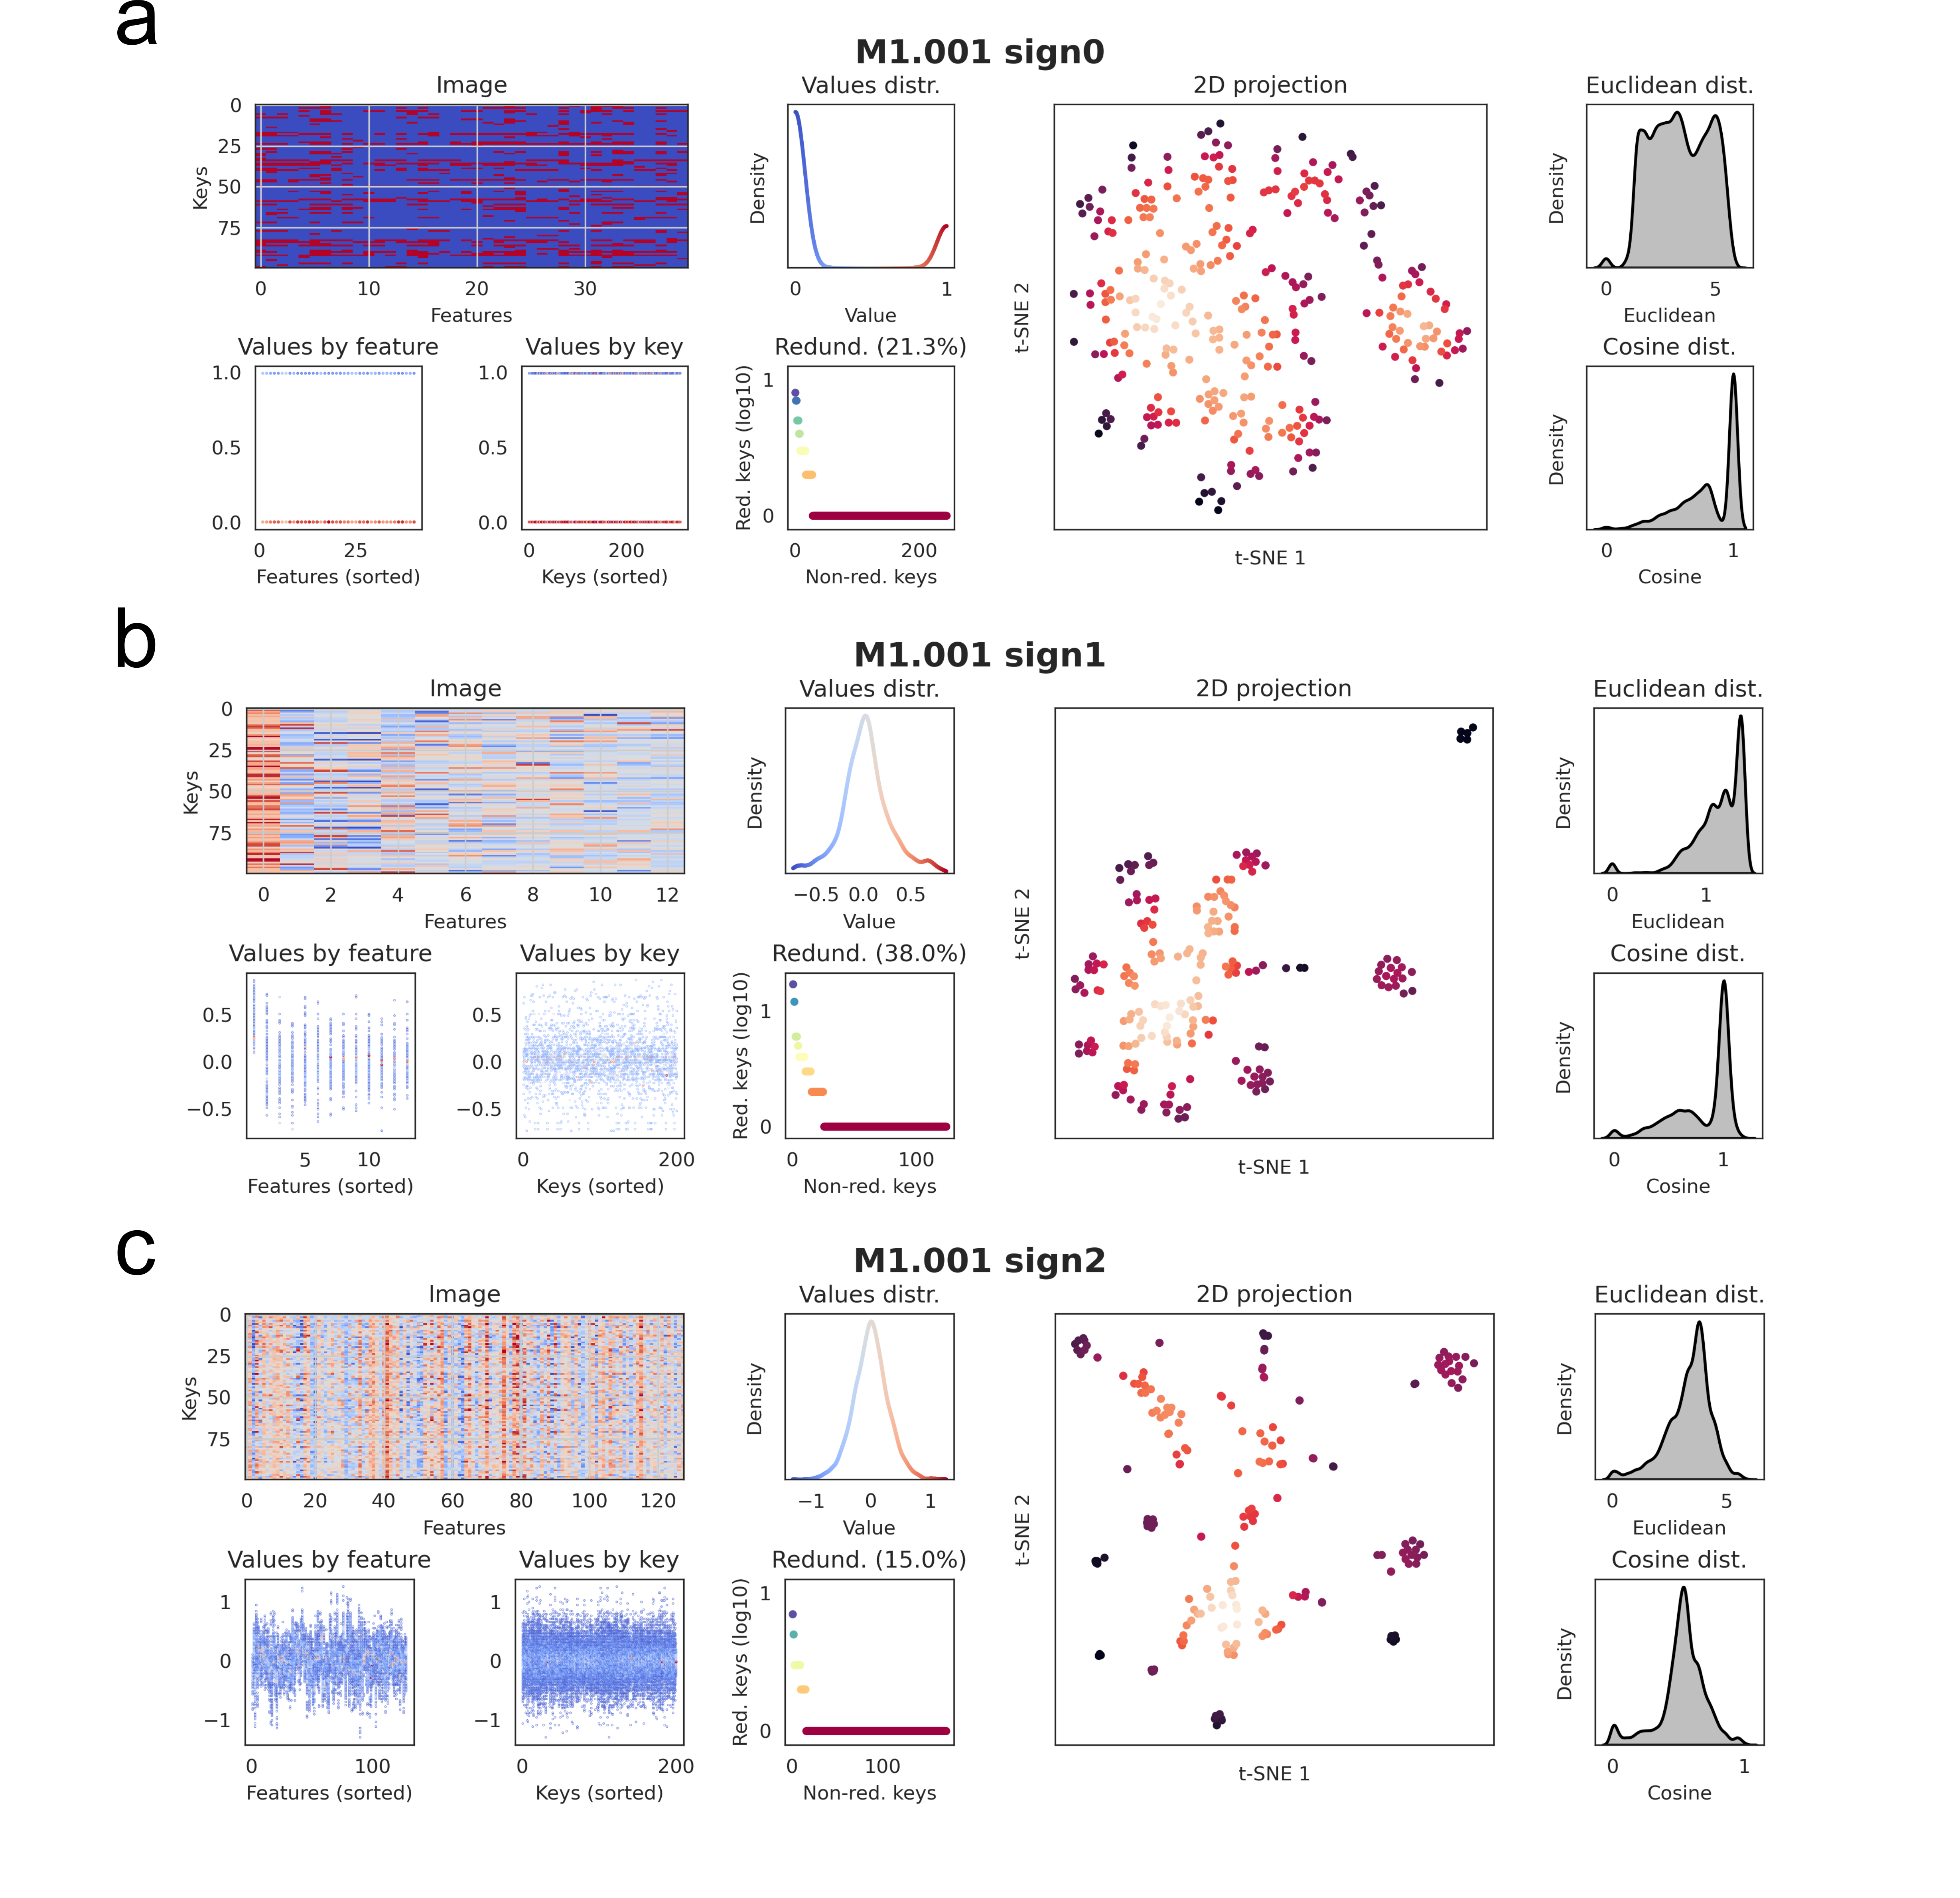
\includegraphics[width=1\linewidth]{figures/Protocols/Supplementary/M1.001_v2.png}
  \caption{
    Diagnosis plots for the M1.001 space
    \textbf{a)} type 0 signatures,
    \textbf{b)} type I signatures,
    \textbf{c)} type II signatures. For further information about diagnosis plots, please see the \hyperref[Supplementary_Protocols_Diagnosis]{Supplementary Information}.
  }
  \label{Protocols_FigS10}
\end{figure}

\begin{figure}[htbp]
  \centering
  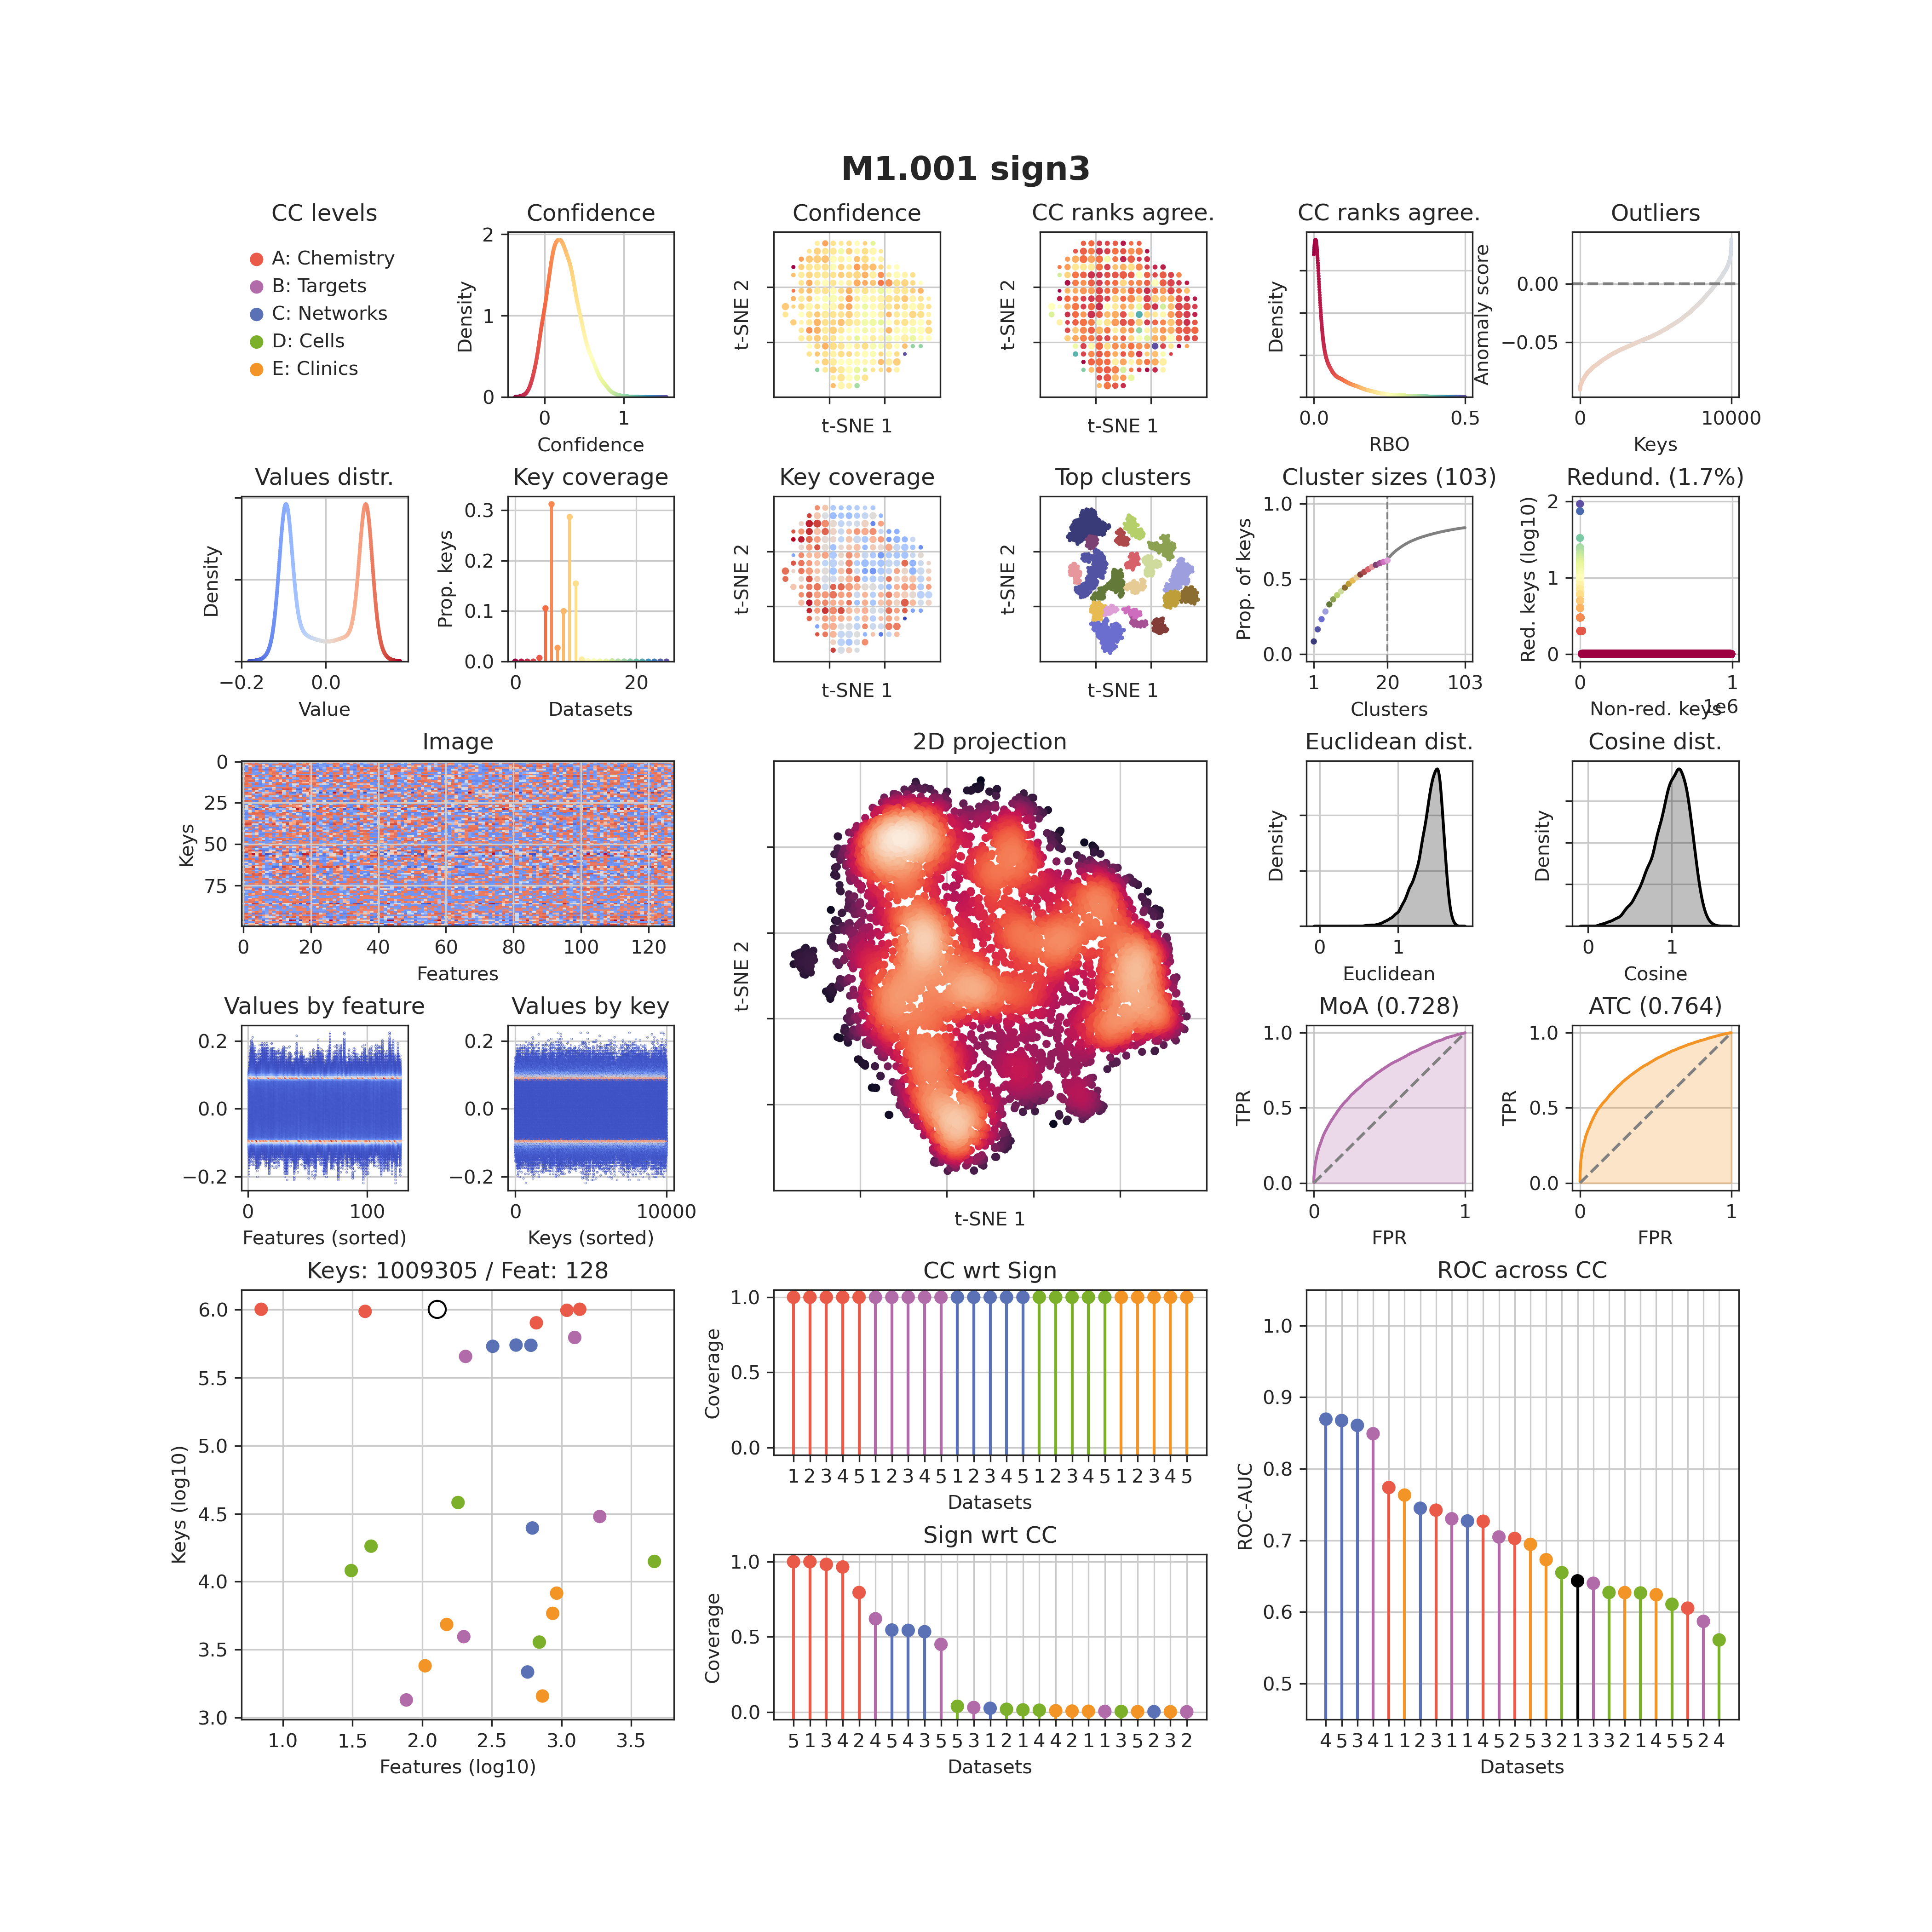
\includegraphics[width=1\linewidth]{figures/Protocols/Supplementary/M1.001_sign3_local_CC_M1_sign0_medium.png}
  \caption{
    Extended diagnosis plots for M1.001 type III signatures. For further information about diagnosis plots, please see the \hyperref[Supplementary_Protocols_Diagnosis]{Supplementary Information} and check our \href{https://gitlabsbnb.irbbarcelona.org/packages/protocols}{Gitlab repository}.
  }
  \label{Protocols_FigS11}
\end{figure}


\clearpage
\phantomsection
\subsection{Interpreting the results: diagnosis plots}
\label{Supplementary_Protocols_Diagnosis}

To assess and monitor data flow at each step of the CC integration pipeline, we have designed several analyses to evaluate the results in a systematic manner. In brief, for each data matrix (compound signatures), a set of diagnosis plots is generated to illustrate the main characteristics of the data. This section includes a comprehensive explanation for each plot.

Examples for small-versioned diagnosis plots are found in Fig \ref{Protocols_FigS1}, Fig \ref{Protocols_FigS4}, Fig \ref{Protocols_FigS7} and Fig \ref{Protocols_FigS10}. From left to right and from top to bottom:
\begin{enumerate}
    \item[\textbullet] Image: heatmap representing the data matrix. Rows are compounds (keys, max. number set to 100), columns are features and colors represent actual values from minimum (blue) to maximum (red).
    \item[\textbullet] Values distribution: density distribution (y-axis) of data values (x-axis) from minimum (blue) to maximum (red). 
    \item[\textbullet] 2D projection: tSNE (t-distributed Stochastic Neighbor Embedding) representation of the data, colored by density. The maximum number of subsampled compounds included in the projection is 10k. 
    \item[\textbullet] Euclidean distribution: density distribution (y-axis) of pairwise Euclidean distances (x-axis). The maximum number of selected compound pairs is set to 10k. 
    \item[\textbullet] Values by feature: numerical values (y-axis) of each feature (x-axis).
    \item[\textbullet] Values by key: numerical values (y-axis) of each compound (key, x-axis).
    \item[\textbullet] Redundancy: for each signature in a non-redundant set of signatures (x-axis), number of compounds (keys, y-axis) having the same exact signature.  
    \item[\textbullet] Cosine distribution: density distribution (y-axis) of pairwise cosine distances (x-axis). The maximum number of selected compound pairs is set to 10k.
\end{enumerate}

The full version of the diagnosis plots provided by the CC comprise additional analysis and comparisons to other CC spaces. Examples of the full version are found in Fig \ref{Protocols_FigS2}, Fig \ref{Protocols_FigS5}, Fig \ref{Protocols_FigS8} and Fig \ref{Protocols_FigS11}. The new plots in the full version are described below from left to right, and from top to bottom:
\begin{enumerate}
    \item[\textbullet]Confidence: density plot (y-axis) of normalized confidence values (x-axis) for the signatures.
    \item[\textbullet]2D projection colored by confidence value: t-SNE representation of the data, colored by their assigned confidence values.
    \item[\textbullet]2D projection colored by CC ranks agreement:  t-SNE representation of the data, colored by their neighbor rank agreement (check next point for additional information).
    \item[\textbullet]CC ranks agreement: distribution of the agreement between compounds neighbors rankings. The lower the score, the lower the agreement among the compounds neighbors rankings.
    \item[\textbullet]Outliers: anomaly score (y-axis) for each signature (x-axis, max. 10k). Signatures with scores above 0 are considered outliers.
    \item[\textbullet]Key Coverage: proportion of compounds in the different CC space datasets (1-25, from A1 to E5, x-axis) found in the new built space.
    \item[\textbullet]2D projection colored by key coverage: t-SNE representation of the data, colored by the compound coverage. Blue indicates higher compound presence across CC spaces.
    \item[\textbullet]Top clusters: 2D representation of the top-20 most populated clusters. The clustering is performed by computing the distances between the signatures and then apply the DBSCAN method.
    \item[\textbullet]Cluster sizes: cumulative proportion of keys (y-axis) assigned to each cluster (x-axis).
    \item[\textbullet]MoA: Recapitulation of the nearest neighbors in the B1.001 space (MoA, type 0 signatures) using the current signature. This recapitulation is quantified by AUROC (Area Under the Receiver Operating Characteristic) values, indicated in the figure title. 
    \item[\textbullet]ATC: Recapitulation of the nearest neighbors in the E1.001 space (therapeutic areas: ATC, type 0 signatures) using the current signature. This recapitulation is quantified by AUROC (Area Under the Receiver Operating Characteristic) values, indicated in the figure title. 
    \item[\textbullet]Keys / Features dimensions: Number of compounds (keys, y-axis) and features (x-axis)for the current signature (white dot), compared to all the other CC spaces. Values were normalized using log10.
    \item[\textbullet]CC wrt Sign: Proportion of keys of the current space that overlaps with the keys of all the other CC spaces. Numbers (ranging from 1 to 5) correspond to each space per level.
    \item[\textbullet]Sign wrt CC: Proportion of the CC keys that overlaps with the current space keys. Numbers (ranging from 1 to 5) correspond to each space per level.
    \item[\textbullet]ROC across CC: Recapitulation of the nearest neighbors of all CC spaces (x-axis, type 0 signatures). This recapitulation is quantified by AUROC (Area Under the Receiver Operating Characteristic) values (y-axis, sorted in descending order). Numbers (ranging from 1 to 5) correspond to each space per level.
\end{enumerate}


\subsection{Downloading the CC bioactivity data}
\label{Supplementary_Protocols_DownloadingData}

To implement all CC functionalities illustrated in this work, we recommend gathering the CC bioactivity data from our web servers using code provided (see \hyperref[Protocols_Methods]{Methods} 3). Since the CC undergoes annual updates, the size of the downloaded files may increase over time, along with the amount of publicly released bioactivity data. To partially overcome long download times or the need for extensive local storage, users may select specific files to download depending on the CC functionality they wish to use. In the following points, we provide a detailed overview of which CC functionalities are related to specific downloadable files, helping users decide what to download.

\phantomsection
\subsubsection{Protocols Essential Functionalities}
\begin{enumerate}
    \item \textbf{Full Type 0 Signatures for Chemical Spaces (A1-5)}: Required for the complete universe functionality. 
    \item \textbf{Reference Type I Signatures for Chemical Spaces (A1-5)}: Required for the complete universe functionality.
    \item \textbf{Reference Type I Models for Chemical Spaces (A1-5)}: Required for the complete universe functionality.
    \item \textbf{Reference Type II Signatures for Chemical Spaces (A1-5)}: Required for the complete universe functionality.
    \item \textbf{Reference Type II Models for Chemical Spaces (A1-5)}: Required for the complete universe functionality.
    \item \textbf{Full Type II Signatures}: Required for generating Type III signatures in a newly created CC space.
    \item \textbf{Full Type III Signatures}: Required for creating medium diagnosis plots for newly generated Type III signatures
    \item \textbf{Metadata}: Required for the generation of medium diagnosis plots.
    
\end{enumerate}

\subsubsection{Additional signatures}

\textbf{Full Type 0, I or II signatures} are necessary for generating medium diagnosis plots for newly created Type 0, I or II signatures. For this protocol, small diagnosis plots are provided for these signature types. 

If users want to evaluate the recapitulation of the raw CC bioactivity data (i.e. type 0 signatures) by means of generated signatures (e.g. type III signatures of a newly created space), they will need to download Full type 0 signatures for all CC spaces (+20GB) and adjust the diagnosis plot code accordingly (i.e. \textit{ref\_cctype=’sign0’}).

\subsubsection{Reduced Data Version for users}

For users not interested in the complete universe functionality, only the \textbf{Full Type II signatures} (for creating Type III signatures) and the \textbf{Full Type III signatures }(for diagnosis) are necessary. 

